% Options for packages loaded elsewhere
\PassOptionsToPackage{unicode}{hyperref}
\PassOptionsToPackage{hyphens}{url}
%
\documentclass[
]{article}
\usepackage{lmodern}
\usepackage{amssymb,amsmath}
\usepackage{ifxetex,ifluatex}
\ifnum 0\ifxetex 1\fi\ifluatex 1\fi=0 % if pdftex
  \usepackage[T1]{fontenc}
  \usepackage[utf8]{inputenc}
  \usepackage{textcomp} % provide euro and other symbols
\else % if luatex or xetex
  \usepackage{unicode-math}
  \defaultfontfeatures{Scale=MatchLowercase}
  \defaultfontfeatures[\rmfamily]{Ligatures=TeX,Scale=1}
\fi
% Use upquote if available, for straight quotes in verbatim environments
\IfFileExists{upquote.sty}{\usepackage{upquote}}{}
\IfFileExists{microtype.sty}{% use microtype if available
  \usepackage[]{microtype}
  \UseMicrotypeSet[protrusion]{basicmath} % disable protrusion for tt fonts
}{}
\makeatletter
\@ifundefined{KOMAClassName}{% if non-KOMA class
  \IfFileExists{parskip.sty}{%
    \usepackage{parskip}
  }{% else
    \setlength{\parindent}{0pt}
    \setlength{\parskip}{6pt plus 2pt minus 1pt}}
}{% if KOMA class
  \KOMAoptions{parskip=half}}
\makeatother
\usepackage{xcolor}
\IfFileExists{xurl.sty}{\usepackage{xurl}}{} % add URL line breaks if available
\IfFileExists{bookmark.sty}{\usepackage{bookmark}}{\usepackage{hyperref}}
\hypersetup{
  pdftitle={Anzahl Resistenzen und einfache plots},
  hidelinks,
  pdfcreator={LaTeX via pandoc}}
\urlstyle{same} % disable monospaced font for URLs
\usepackage[margin=0.5cm]{geometry}
\usepackage{color}
\usepackage{fancyvrb}
\newcommand{\VerbBar}{|}
\newcommand{\VERB}{\Verb[commandchars=\\\{\}]}
\DefineVerbatimEnvironment{Highlighting}{Verbatim}{commandchars=\\\{\}}
% Add ',fontsize=\small' for more characters per line
\usepackage{framed}
\definecolor{shadecolor}{RGB}{248,248,248}
\newenvironment{Shaded}{\begin{snugshade}}{\end{snugshade}}
\newcommand{\AlertTok}[1]{\textcolor[rgb]{0.94,0.16,0.16}{#1}}
\newcommand{\AnnotationTok}[1]{\textcolor[rgb]{0.56,0.35,0.01}{\textbf{\textit{#1}}}}
\newcommand{\AttributeTok}[1]{\textcolor[rgb]{0.77,0.63,0.00}{#1}}
\newcommand{\BaseNTok}[1]{\textcolor[rgb]{0.00,0.00,0.81}{#1}}
\newcommand{\BuiltInTok}[1]{#1}
\newcommand{\CharTok}[1]{\textcolor[rgb]{0.31,0.60,0.02}{#1}}
\newcommand{\CommentTok}[1]{\textcolor[rgb]{0.56,0.35,0.01}{\textit{#1}}}
\newcommand{\CommentVarTok}[1]{\textcolor[rgb]{0.56,0.35,0.01}{\textbf{\textit{#1}}}}
\newcommand{\ConstantTok}[1]{\textcolor[rgb]{0.00,0.00,0.00}{#1}}
\newcommand{\ControlFlowTok}[1]{\textcolor[rgb]{0.13,0.29,0.53}{\textbf{#1}}}
\newcommand{\DataTypeTok}[1]{\textcolor[rgb]{0.13,0.29,0.53}{#1}}
\newcommand{\DecValTok}[1]{\textcolor[rgb]{0.00,0.00,0.81}{#1}}
\newcommand{\DocumentationTok}[1]{\textcolor[rgb]{0.56,0.35,0.01}{\textbf{\textit{#1}}}}
\newcommand{\ErrorTok}[1]{\textcolor[rgb]{0.64,0.00,0.00}{\textbf{#1}}}
\newcommand{\ExtensionTok}[1]{#1}
\newcommand{\FloatTok}[1]{\textcolor[rgb]{0.00,0.00,0.81}{#1}}
\newcommand{\FunctionTok}[1]{\textcolor[rgb]{0.00,0.00,0.00}{#1}}
\newcommand{\ImportTok}[1]{#1}
\newcommand{\InformationTok}[1]{\textcolor[rgb]{0.56,0.35,0.01}{\textbf{\textit{#1}}}}
\newcommand{\KeywordTok}[1]{\textcolor[rgb]{0.13,0.29,0.53}{\textbf{#1}}}
\newcommand{\NormalTok}[1]{#1}
\newcommand{\OperatorTok}[1]{\textcolor[rgb]{0.81,0.36,0.00}{\textbf{#1}}}
\newcommand{\OtherTok}[1]{\textcolor[rgb]{0.56,0.35,0.01}{#1}}
\newcommand{\PreprocessorTok}[1]{\textcolor[rgb]{0.56,0.35,0.01}{\textit{#1}}}
\newcommand{\RegionMarkerTok}[1]{#1}
\newcommand{\SpecialCharTok}[1]{\textcolor[rgb]{0.00,0.00,0.00}{#1}}
\newcommand{\SpecialStringTok}[1]{\textcolor[rgb]{0.31,0.60,0.02}{#1}}
\newcommand{\StringTok}[1]{\textcolor[rgb]{0.31,0.60,0.02}{#1}}
\newcommand{\VariableTok}[1]{\textcolor[rgb]{0.00,0.00,0.00}{#1}}
\newcommand{\VerbatimStringTok}[1]{\textcolor[rgb]{0.31,0.60,0.02}{#1}}
\newcommand{\WarningTok}[1]{\textcolor[rgb]{0.56,0.35,0.01}{\textbf{\textit{#1}}}}
\usepackage{graphicx,grffile}
\makeatletter
\def\maxwidth{\ifdim\Gin@nat@width>\linewidth\linewidth\else\Gin@nat@width\fi}
\def\maxheight{\ifdim\Gin@nat@height>\textheight\textheight\else\Gin@nat@height\fi}
\makeatother
% Scale images if necessary, so that they will not overflow the page
% margins by default, and it is still possible to overwrite the defaults
% using explicit options in \includegraphics[width, height, ...]{}
\setkeys{Gin}{width=\maxwidth,height=\maxheight,keepaspectratio}
% Set default figure placement to htbp
\makeatletter
\def\fps@figure{htbp}
\makeatother
\setlength{\emergencystretch}{3em} % prevent overfull lines
\providecommand{\tightlist}{%
  \setlength{\itemsep}{0pt}\setlength{\parskip}{0pt}}
\setcounter{secnumdepth}{-\maxdimen} % remove section numbering

\title{Anzahl Resistenzen und einfache plots}
\author{}
\date{\vspace{-2.5em}23.03.2022}

\begin{document}
\maketitle

Es darf kein Verzeichnis NResistenzen\_files/ geben, sonst werden nicht
die neuen plots gespeichert!

\hypertarget{bibliotheken-laden-hilfsfunktion}{%
\section{Bibliotheken laden,
Hilfsfunktion}\label{bibliotheken-laden-hilfsfunktion}}

\begin{Shaded}
\begin{Highlighting}[]
\KeywordTok{library}\NormalTok{(ggplot2)     }\CommentTok{# moderne plots}

\NormalTok{debug <-}\StringTok{ }\NormalTok{T           }\CommentTok{# debug printout}
\NormalTok{debug <-}\StringTok{ }\NormalTok{F           }\CommentTok{# kein debug printout}
\NormalTok{Log <-}\StringTok{ }\ControlFlowTok{function}\NormalTok{(string) \{}
  \ControlFlowTok{if}\NormalTok{(debug)\{}\KeywordTok{print}\NormalTok{(string)\}  }
\NormalTok{\}}
\end{Highlighting}
\end{Shaded}

\hypertarget{my-schicht-festlegen}{%
\section{MY Schicht Festlegen}\label{my-schicht-festlegen}}

Die letzte Zeile zählt!

\begin{Shaded}
\begin{Highlighting}[]
\NormalTok{Schicht <-}\StringTok{ "U"}         \CommentTok{# Un-stratified}
\NormalTok{Schicht <-}\StringTok{ "LE8000"}    \CommentTok{# Less than or Equal to 8000}
\NormalTok{Schicht <-}\StringTok{ "GT8000"}    \CommentTok{# Greater Than 8000}
\end{Highlighting}
\end{Shaded}

\hypertarget{resistenzen.rmd-erzeugte-resistenzenschicht.csv-dieses-einlesen}{%
\section{Resistenzen.Rmd erzeugte Resistenzen{[}Schicht{]}.csv, dieses
einlesen}\label{resistenzen.rmd-erzeugte-resistenzenschicht.csv-dieses-einlesen}}

Und evtl. ansehen

\begin{Shaded}
\begin{Highlighting}[]
\NormalTok{FileIn <-}\StringTok{ }\KeywordTok{paste}\NormalTok{( }\StringTok{"Resistenzen"}\NormalTok{,Schicht,}\StringTok{".csv"}\NormalTok{ , }\DataTypeTok{sep=}\StringTok{""}\NormalTok{ )  }\CommentTok{# Fileout ist nur N davorgehängt}
\NormalTok{Resistenzen <-}\StringTok{ }\KeywordTok{read.csv}\NormalTok{(FileIn)}

\CommentTok{# csv schreiben fügt vorne Index-Spalte an; diese entfernen :}
\NormalTok{Resistenzen[,}\DecValTok{1}\NormalTok{] <-}\StringTok{ }\OtherTok{NULL}                      

\ControlFlowTok{if}\NormalTok{(debug)\{}\KeywordTok{View}\NormalTok{(Resistenzen)\}}
\end{Highlighting}
\end{Shaded}

\hypertarget{resistenzen-pro-betrieb}{%
\section{Resistenzen pro Betrieb}\label{resistenzen-pro-betrieb}}

Resistenzen pro Betrieb in neuer Tabelle ``NResistenzen'' zählen,
Multirestenz dokumentieren und als NResistenzen.csv ausschreiben

\begin{Shaded}
\begin{Highlighting}[]
\NormalTok{ResRow  <-}\StringTok{ }\KeywordTok{nrow}\NormalTok{(Resistenzen)  }\CommentTok{# Zeilen Resistenzen : 4 pro Betrieb}
\NormalTok{NResRow <-}\StringTok{ }\NormalTok{ResRow}\OperatorTok{/}\DecValTok{4}           \CommentTok{# Zeilen NResistenzen : 1 pro Betrieb}
\NormalTok{NAntib  <-}\StringTok{ }\DecValTok{15}                 \CommentTok{# wir untersuchen 15 Antibiotika (wird von Resistenzen.Rmd so aus 2 Excel files eingelesen)}

\NormalTok{NResistenzen <-}\StringTok{ }\NormalTok{Resistenzen[}\DecValTok{0}\NormalTok{,]                          }\CommentTok{# header wie"Resistenzen"}
\ControlFlowTok{for}\NormalTok{(line }\ControlFlowTok{in} \DecValTok{1}\OperatorTok{:}\NormalTok{NResRow)\{                                  }\CommentTok{# 1 bis 60, aber 30 fehlt}
\NormalTok{  i <-}\StringTok{ }\NormalTok{(line }\OperatorTok{-}\StringTok{ }\DecValTok{1}\NormalTok{)}\OperatorTok{*}\DecValTok{4} \OperatorTok{+}\StringTok{ }\DecValTok{1}
\NormalTok{  NResistenzen[line,] <-}\StringTok{ }\NormalTok{Resistenzen[(line }\OperatorTok{-}\StringTok{ }\DecValTok{1}\NormalTok{)}\OperatorTok{*}\DecValTok{4} \OperatorTok{+}\StringTok{ }\DecValTok{1}\NormalTok{,]  }\CommentTok{# WM.group etc. kopieren}
\NormalTok{  NResistenzen[line,}\DecValTok{2}\OperatorTok{:}\NormalTok{(NAntib}\OperatorTok{+}\DecValTok{1}\NormalTok{)] <-}\StringTok{ }\DecValTok{0}                   \CommentTok{# aber Antibiotika auf 0 setzen : hier später Resistenzen zählen}
\NormalTok{\}}
\ControlFlowTok{for}\NormalTok{(col }\ControlFlowTok{in} \DecValTok{2}\OperatorTok{:}\NormalTok{(NAntib}\OperatorTok{+}\DecValTok{1}\NormalTok{))\{}
\NormalTok{  NResistenzen[,col] <-}\StringTok{  }\KeywordTok{as.numeric}\NormalTok{(NResistenzen[,col])  }\CommentTok{# muss immer noch in type double konvertieren}
\NormalTok{\}}
\ControlFlowTok{if}\NormalTok{(debug)\{}\KeywordTok{View}\NormalTok{(NResistenzen)\} }

\CommentTok{# für jedes Antibiotikum Resistenzen über die 4 Proben zählen, also mögliche Werte 0-4 :}
\ControlFlowTok{for}\NormalTok{(i }\ControlFlowTok{in} \DecValTok{1}\OperatorTok{:}\NormalTok{ResRow)\{                             }\CommentTok{# Liniennummer (Betriebe in 4er Gruppen) für dataframe Resistenzen}
  \KeywordTok{Log}\NormalTok{(}\KeywordTok{paste}\NormalTok{(}\StringTok{"i="}\NormalTok{,i))}
  
\NormalTok{  line <-}\StringTok{ }\KeywordTok{floor}\NormalTok{((i}\DecValTok{-1}\NormalTok{)}\OperatorTok{/}\DecValTok{4}\NormalTok{)}\OperatorTok{+}\DecValTok{1}                      \CommentTok{# Liniennummer für dataframe NResistenzen}
  
  \ControlFlowTok{for}\NormalTok{(j }\ControlFlowTok{in} \DecValTok{2}\OperatorTok{:}\NormalTok{(NAntib}\OperatorTok{+}\DecValTok{1}\NormalTok{))\{                            }\CommentTok{# Spaltennummer: Antibiotikum}

    \ControlFlowTok{if}\NormalTok{(}\KeywordTok{substr}\NormalTok{(Resistenzen[i,j],}\DecValTok{1}\NormalTok{,}\DecValTok{1}\NormalTok{)}\OperatorTok{==}\StringTok{">"}\NormalTok{)\{   }\CommentTok{# wenn Resistenz}
      \KeywordTok{Log}\NormalTok{(}\KeywordTok{paste}\NormalTok{(}\StringTok{"  NResistenzen["}\NormalTok{,line,j,}\StringTok{"]="}\NormalTok{,NResistenzen[line,j],}\KeywordTok{typeof}\NormalTok{(NResistenzen[line,j]) ))}
\NormalTok{      NResistenzen[line,j] <-}\StringTok{ }\NormalTok{NResistenzen[line,j] }\OperatorTok{+}\StringTok{ }\DecValTok{1}  \CommentTok{# gef. Resistenz zählen}
\NormalTok{\} \} \} }

\NormalTok{NResistenzen}\OperatorTok{$}\NormalTok{NRes   <-}\StringTok{ }\KeywordTok{rep}\NormalTok{(}\DecValTok{0}\NormalTok{,NResRow)  }\CommentTok{# neue Spalte, zählt für jeden Betrieb Resistenzen über Antibiotika; erstmal 0}
\NormalTok{NResistenzen}\OperatorTok{$}\NormalTok{MultiR <-}\StringTok{ }\KeywordTok{rep}\NormalTok{(F,NResRow)  }\CommentTok{# neue Spalte, dokumentiert für jeden Betrieb Multiresistenz; erstmal False}
\ControlFlowTok{for}\NormalTok{(line }\ControlFlowTok{in} \DecValTok{1}\OperatorTok{:}\NormalTok{NResRow)\{              }\CommentTok{# 1 bis 60, aber 30 fehlt}
  \ControlFlowTok{for}\NormalTok{(col }\ControlFlowTok{in} \DecValTok{2}\OperatorTok{:}\NormalTok{(NAntib}\OperatorTok{+}\DecValTok{1}\NormalTok{))\{}
    \ControlFlowTok{if}\NormalTok{(NResistenzen[line,col] }\OperatorTok{>}\StringTok{ }\DecValTok{0}\NormalTok{)\{}
\NormalTok{      NResistenzen[line,}\StringTok{"NRes"}\NormalTok{] <-}\StringTok{ }\NormalTok{NResistenzen[line,}\StringTok{"NRes"}\NormalTok{]}\OperatorTok{+}\DecValTok{1}  \CommentTok{# Resistenz zählen}
\NormalTok{    \}}
\NormalTok{  \}}
  \ControlFlowTok{if}\NormalTok{(NResistenzen[line,}\StringTok{"NRes"}\NormalTok{] }\OperatorTok{>=}\StringTok{ }\DecValTok{3}\NormalTok{)\{  }\CommentTok{# Multiresistenz heisst mind. 3 Resistenzen}
\NormalTok{    NResistenzen[line,}\StringTok{"MultiR"}\NormalTok{] <-}\StringTok{ }\NormalTok{T}
\NormalTok{  \}}
\NormalTok{\}}
\ControlFlowTok{if}\NormalTok{(debug)\{}\KeywordTok{View}\NormalTok{(NResistenzen)\}}
\KeywordTok{write.csv}\NormalTok{(NResistenzen, }\KeywordTok{paste}\NormalTok{( }\StringTok{"N"}\NormalTok{, FileIn , }\DataTypeTok{sep=}\StringTok{""}\NormalTok{ ))}
\end{Highlighting}
\end{Shaded}

\hypertarget{numerische-und-ordinale-unabhuxe4ngige-variablen}{%
\section{Numerische und Ordinale Unabhängige
Variablen}\label{numerische-und-ordinale-unabhuxe4ngige-variablen}}

\begin{Shaded}
\begin{Highlighting}[]
\NormalTok{graphisch2 <-}\StringTok{ }\ControlFlowTok{function}\NormalTok{(gruppe, join, antibiotikum) \{}
\NormalTok{  group <-}\StringTok{ }\NormalTok{Resistenzen[,gruppe ] }
\NormalTok{  antib      <-}\StringTok{ }\NormalTok{Resistenzen[,antibiotikum ]}

\NormalTok{  X <-}\StringTok{ }\KeywordTok{c}\NormalTok{()}
\NormalTok{  Y <-}\StringTok{ }\KeywordTok{c}\NormalTok{()}
  \ControlFlowTok{for}\NormalTok{(i }\ControlFlowTok{in} \DecValTok{1}\OperatorTok{:}\NormalTok{ResRow)\{                      }\CommentTok{# Liniennummer für dataframe Resistenzen}
\NormalTok{    x <-}\StringTok{ }\KeywordTok{as.numeric}\NormalTok{(group[i])              }\CommentTok{# [,na.rm=TRUE) hilft nicht weil's "NA" ist, nicht NA]}
    \ControlFlowTok{if}\NormalTok{(}\KeywordTok{substr}\NormalTok{(antib[i],}\DecValTok{1}\NormalTok{,}\DecValTok{1}\NormalTok{) }\OperatorTok{==}\StringTok{ ">"}\NormalTok{)\{       }\CommentTok{# wenn Resistenz}
      
\NormalTok{      pos <-}\StringTok{ }\KeywordTok{match}\NormalTok{(x,X)                   }
      \ControlFlowTok{if}\NormalTok{(}\KeywordTok{is.na}\NormalTok{(pos))\{}
\NormalTok{        X <-}\StringTok{ }\KeywordTok{c}\NormalTok{(X,x)    }\CommentTok{# faster: pre-allocate+assign,}
\NormalTok{        Y <-}\StringTok{ }\KeywordTok{c}\NormalTok{(Y,}\DecValTok{1}\NormalTok{)    }\CommentTok{# in this way vector copied in every iteration}
\NormalTok{      \} }\ControlFlowTok{else}\NormalTok{ \{}
\NormalTok{        Y[pos] <-}\StringTok{ }\NormalTok{Y[pos] }\OperatorTok{+}\StringTok{ }\DecValTok{1}
\NormalTok{      \}}
\NormalTok{    \}}
\NormalTok{  \}  }

\NormalTok{  df <-}\StringTok{ }\KeywordTok{data.frame}\NormalTok{(X,Y)}
\NormalTok{  ylab <-}\StringTok{ }\KeywordTok{paste}\NormalTok{(antibiotikum,}\StringTok{"- Resistenzen"}\NormalTok{)}
  
  \ControlFlowTok{if}\NormalTok{( gruppe }\OperatorTok{==}\StringTok{ "WM.group"}\NormalTok{ )\{xlab <-}\StringTok{ "Wastemilk-Gruppe"}\NormalTok{\}}
  \ControlFlowTok{if}\NormalTok{( gruppe }\OperatorTok{==}\StringTok{ "OLS.group"}\NormalTok{)\{xlab <-}\StringTok{ "Other LiveStock-Gruppe"}\NormalTok{\}            }
  \ControlFlowTok{if}\NormalTok{( gruppe }\OperatorTok{==}\StringTok{ "IAC.group"}\NormalTok{)\{xlab <-}\StringTok{ "Ill Animals in Calving box-Gruppe"}\NormalTok{\}}
  \CommentTok{### Neue binäre hier dazufügen }\AlertTok{###}

  \ControlFlowTok{if}\NormalTok{( gruppe }\OperatorTok{==}\StringTok{ "HSC.group"}\NormalTok{)\{xlab <-}\StringTok{ "Husbandry System Calves-Gruppe"}\NormalTok{\}   }
  \CommentTok{### Neue nominale hier dazufügen }\AlertTok{###}
  
  \ControlFlowTok{if}\NormalTok{( gruppe }\OperatorTok{==}\StringTok{ "MY"}\NormalTok{       )\{xlab <-}\StringTok{ "meanMY/cow"}\NormalTok{\}}
  \ControlFlowTok{if}\NormalTok{( gruppe }\OperatorTok{==}\StringTok{ "SCC"}\NormalTok{      )\{xlab <-}\StringTok{ "mean SCC/11mo"}\NormalTok{\}          }
  \ControlFlowTok{if}\NormalTok{( gruppe }\OperatorTok{==}\StringTok{ "CBC"}\NormalTok{      )\{xlab <-}\StringTok{ "calvingbox_clean"}\NormalTok{\}    }
  \ControlFlowTok{if}\NormalTok{( gruppe }\OperatorTok{==}\StringTok{ "DIA"}\NormalTok{      )\{xlab <-}\StringTok{ "IN_diarrhea<30d"}\NormalTok{\}               }
  \CommentTok{### Neue numerische hier dazufügen }\AlertTok{###}

\NormalTok{  min <-}\StringTok{ }\KeywordTok{min}\NormalTok{(}\KeywordTok{as.numeric}\NormalTok{(Resistenzen[,gruppe]), }\DataTypeTok{na.rm=}\NormalTok{T)}
\NormalTok{  max <-}\StringTok{ }\KeywordTok{max}\NormalTok{(}\KeywordTok{as.numeric}\NormalTok{(Resistenzen[,gruppe]), }\DataTypeTok{na.rm=}\NormalTok{T)}
  
\NormalTok{  puffer <-}\StringTok{ }\NormalTok{(max }\OperatorTok{-}\StringTok{ }\NormalTok{min)}\OperatorTok{/}\DecValTok{20}     
\NormalTok{  min <-}\StringTok{ }\NormalTok{min }\OperatorTok{-}\StringTok{ }\NormalTok{puffer       }\CommentTok{# links und rechts 5% freier Platz}
\NormalTok{  max <-}\StringTok{ }\NormalTok{max }\OperatorTok{+}\StringTok{ }\NormalTok{puffer}
  
  \KeywordTok{print}\NormalTok{( }\KeywordTok{ggplot}\NormalTok{(df, }\KeywordTok{aes}\NormalTok{(X, Y)) }\OperatorTok{+}\StringTok{ }
\StringTok{    }\KeywordTok{geom_point}\NormalTok{() }\OperatorTok{+}
\StringTok{    }\KeywordTok{xlim}\NormalTok{(min,max) }\OperatorTok{+}
\StringTok{    }\KeywordTok{xlab}\NormalTok{(xlab) }\OperatorTok{+}\StringTok{ }\KeywordTok{ylab}\NormalTok{(ylab)  }\OperatorTok{+}\StringTok{ }
\StringTok{    }\KeywordTok{ggtitle}\NormalTok{(}\KeywordTok{paste}\NormalTok{(}\StringTok{"Anzahl"}\NormalTok{, ylab, join,xlab))   }
\NormalTok{  )}
\NormalTok{\}}
\end{Highlighting}
\end{Shaded}

\hypertarget{plot-anzahl-der-resistenzen-fuxfcr-verschiedene-antibiotika-numerische-variablen}{%
\section{Plot Anzahl der Resistenzen für verschiedene Antibiotika,
numerische
Variablen}\label{plot-anzahl-der-resistenzen-fuxfcr-verschiedene-antibiotika-numerische-variablen}}

\begin{itemize}
\tightlist
\item
  MERO, AMI, TGC, TAZ COL, keine Resistenzen
\item
  FOT , AZI nur eine (die AZI-CBC und AZI-IAC plots sind korrekterweise
  leer: Diese Resistenz hat NA für CBC und IAC)
\end{itemize}

\begin{Shaded}
\begin{Highlighting}[]
\CommentTok{#   NA warnings interessieren nicht}
 
\NormalTok{numerisch <-}\StringTok{ }\KeywordTok{c}\NormalTok{(}\StringTok{"MY"}\NormalTok{,}\StringTok{"SCC"}\NormalTok{,}\StringTok{"CBC"}\NormalTok{,}\StringTok{"DIA"}\NormalTok{)     }\CommentTok{# untersuchte numerische Variablen  }\AlertTok{###}\CommentTok{ neue numerische hier hinzufügen }\AlertTok{###}
\ControlFlowTok{for}\NormalTok{( group }\ControlFlowTok{in}\NormalTok{ numerisch) \{   }

  \ControlFlowTok{for}\NormalTok{( antib }\ControlFlowTok{in} \KeywordTok{c}\NormalTok{(}\StringTok{"AMP"}\NormalTok{,}\StringTok{"CIP"}\NormalTok{,}\StringTok{"AZI"}\NormalTok{,}\StringTok{"GEN"}\NormalTok{,}\StringTok{"FOT"}\NormalTok{,}\StringTok{"CHL"}\NormalTok{,}\StringTok{"NAL"}\NormalTok{,}\StringTok{"TET"}\NormalTok{,}\StringTok{"TMP"}\NormalTok{,}\StringTok{"SMX"}\NormalTok{) )\{ }
  
    \KeywordTok{graphisch2}\NormalTok{(group,}\StringTok{"für geg."}\NormalTok{,antib)  }
    \KeywordTok{print}\NormalTok{(}\StringTok{""}\NormalTok{)}
\NormalTok{  \} }
  \KeywordTok{print}\NormalTok{(}\StringTok{"--------------------------------------------------------"}\NormalTok{)}
\NormalTok{\}}
\end{Highlighting}
\end{Shaded}

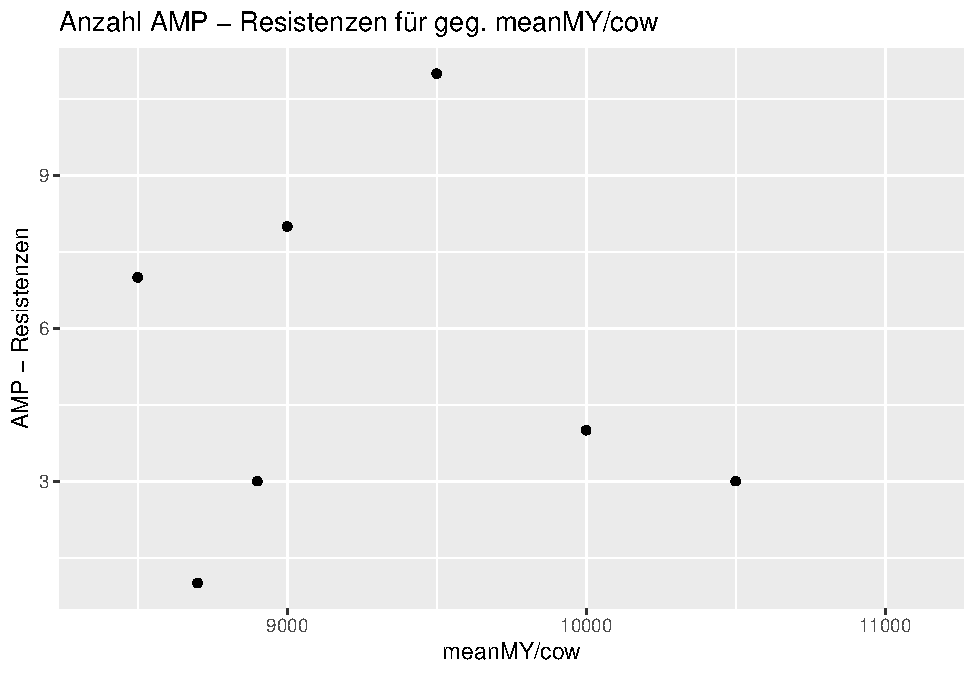
\includegraphics{NResistenzen_files/figure-latex/unnamed-chunk-6-1.pdf}

\begin{verbatim}
## [1] ""
\end{verbatim}

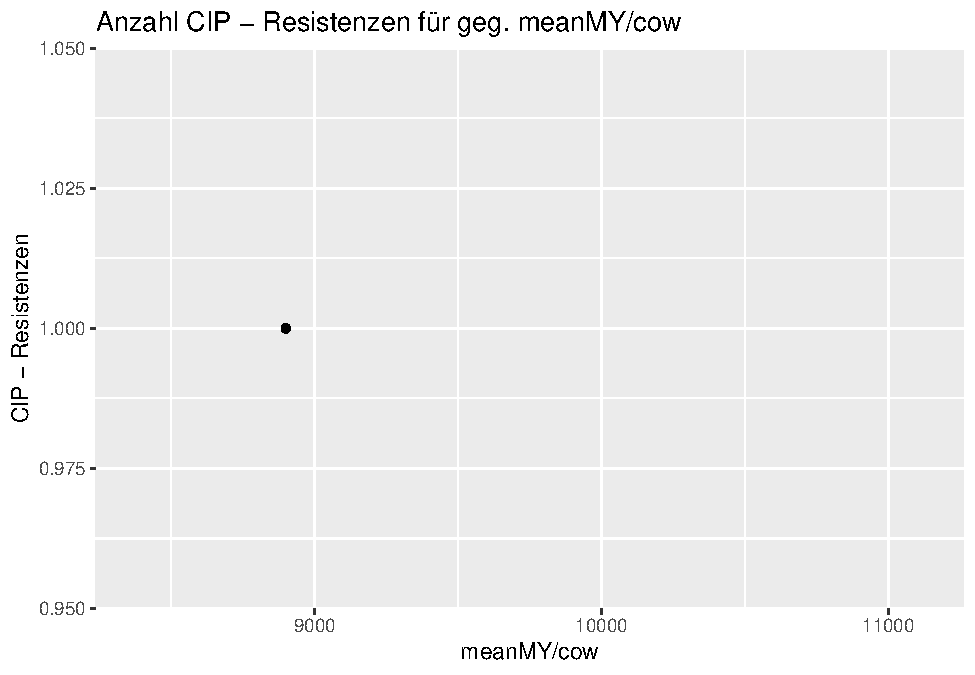
\includegraphics{NResistenzen_files/figure-latex/unnamed-chunk-6-2.pdf}

\begin{verbatim}
## [1] ""
\end{verbatim}

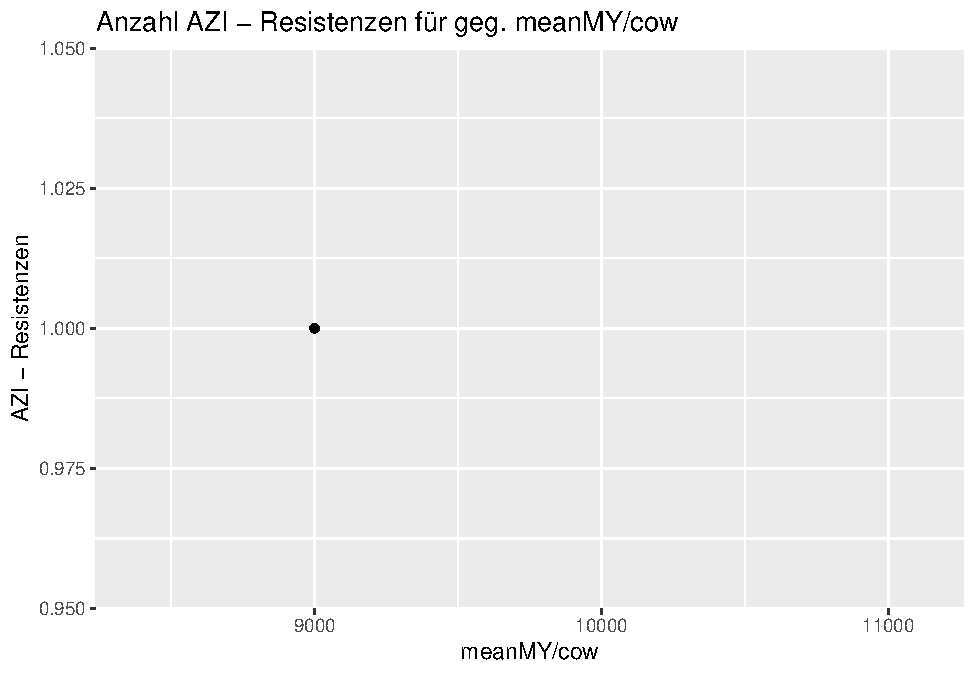
\includegraphics{NResistenzen_files/figure-latex/unnamed-chunk-6-3.pdf}

\begin{verbatim}
## [1] ""
\end{verbatim}

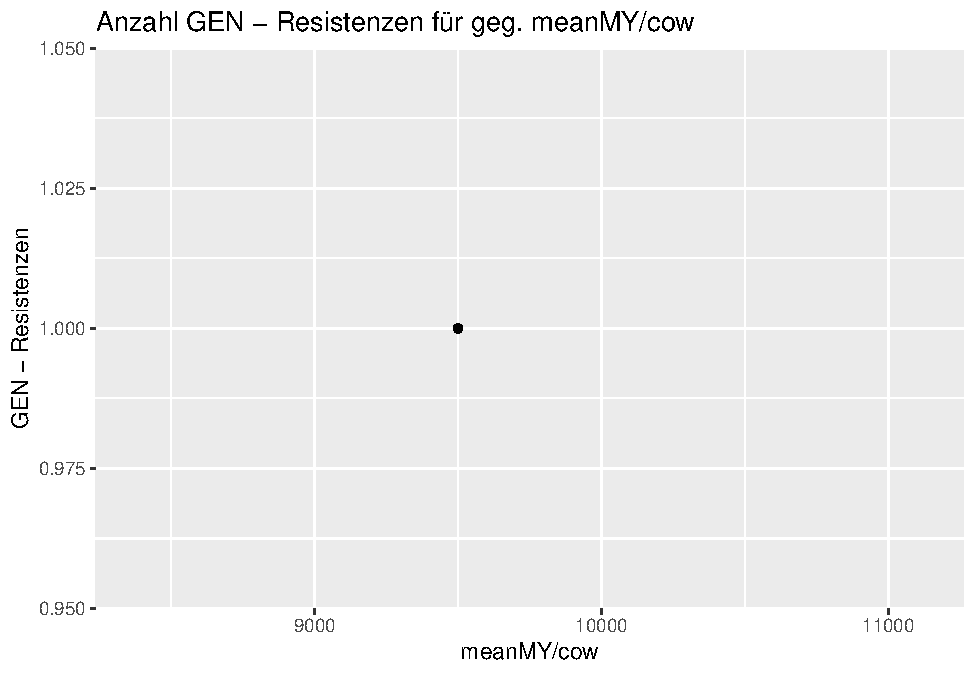
\includegraphics{NResistenzen_files/figure-latex/unnamed-chunk-6-4.pdf}

\begin{verbatim}
## [1] ""
\end{verbatim}

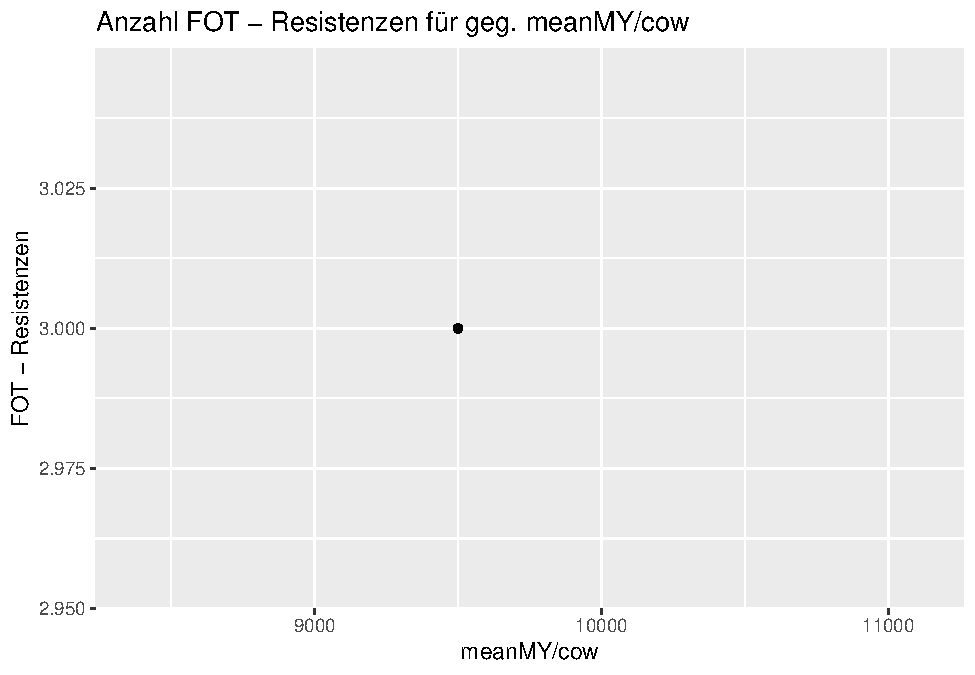
\includegraphics{NResistenzen_files/figure-latex/unnamed-chunk-6-5.pdf}

\begin{verbatim}
## [1] ""
\end{verbatim}

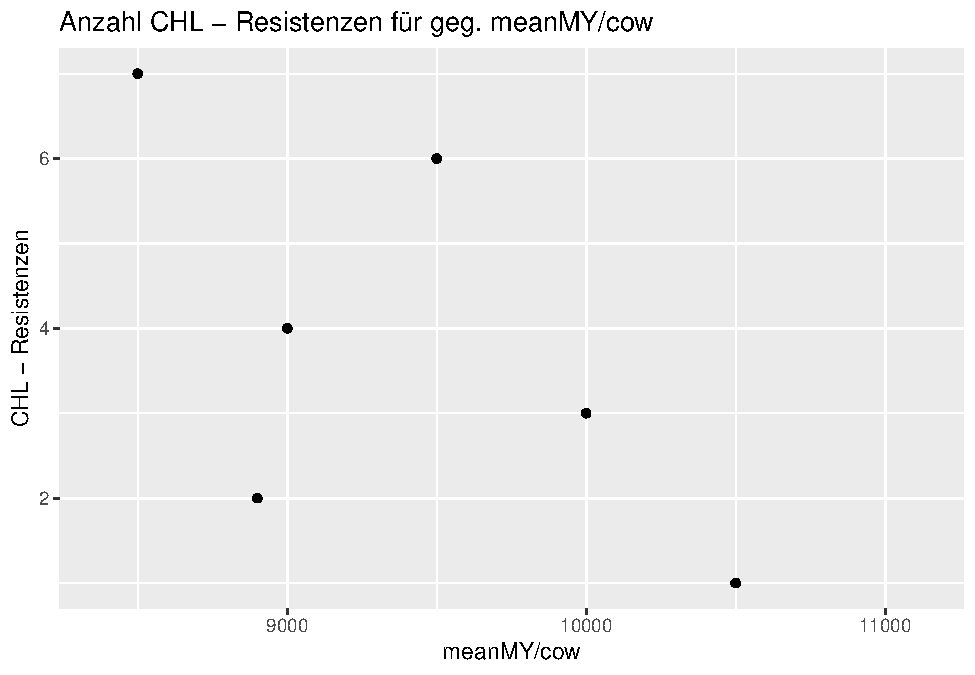
\includegraphics{NResistenzen_files/figure-latex/unnamed-chunk-6-6.pdf}

\begin{verbatim}
## [1] ""
\end{verbatim}

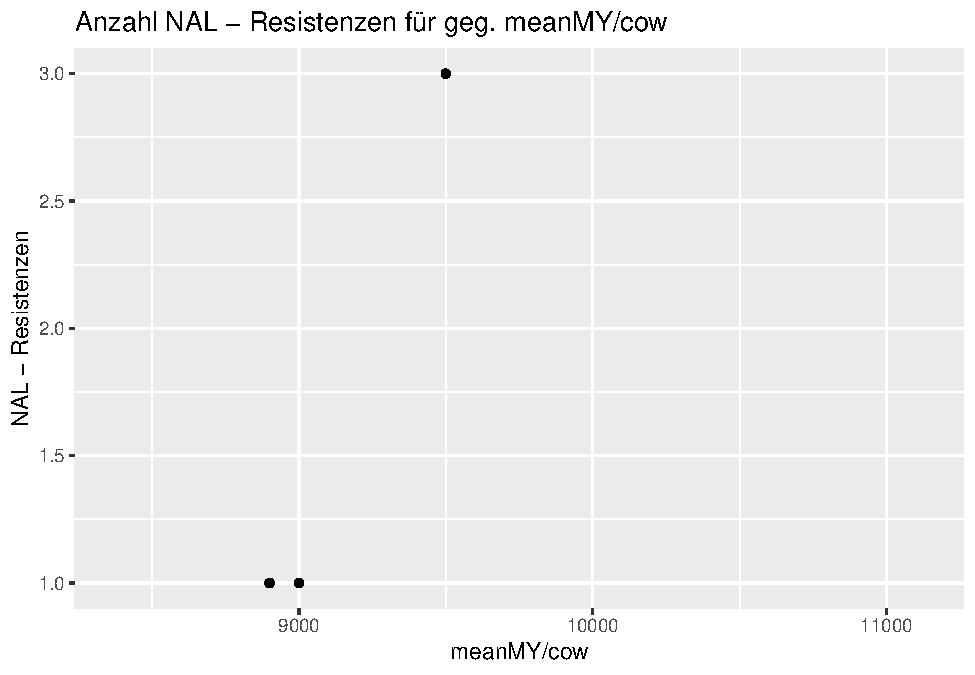
\includegraphics{NResistenzen_files/figure-latex/unnamed-chunk-6-7.pdf}

\begin{verbatim}
## [1] ""
\end{verbatim}

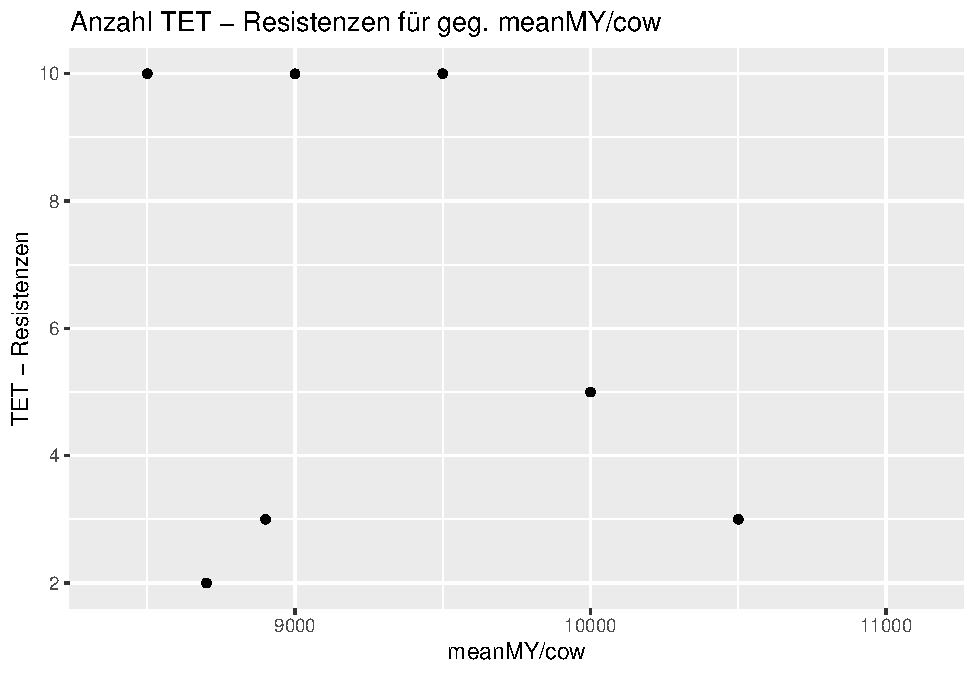
\includegraphics{NResistenzen_files/figure-latex/unnamed-chunk-6-8.pdf}

\begin{verbatim}
## [1] ""
\end{verbatim}

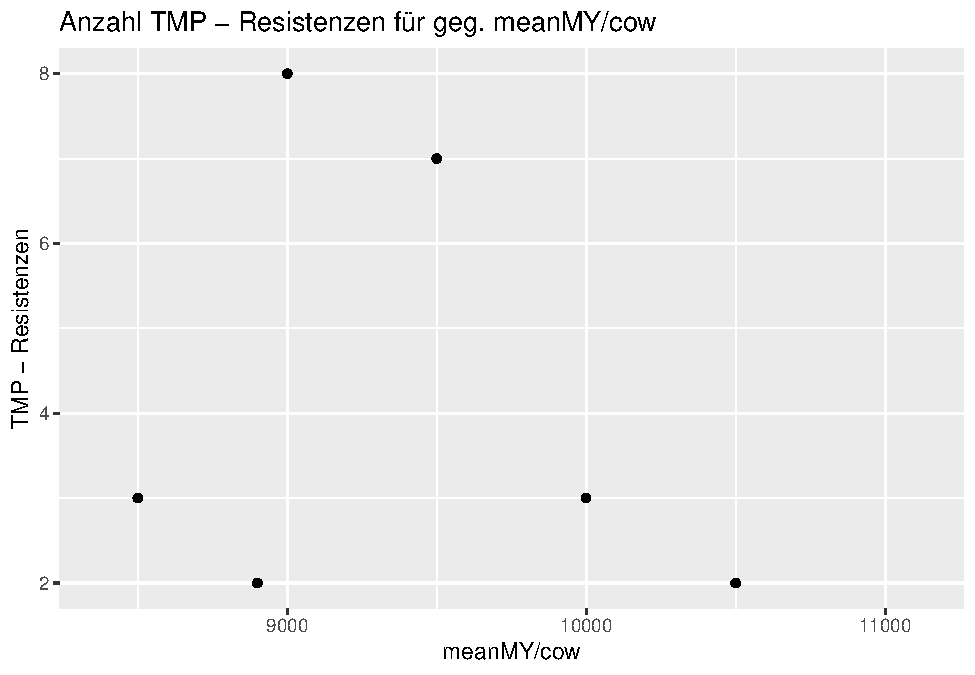
\includegraphics{NResistenzen_files/figure-latex/unnamed-chunk-6-9.pdf}

\begin{verbatim}
## [1] ""
\end{verbatim}

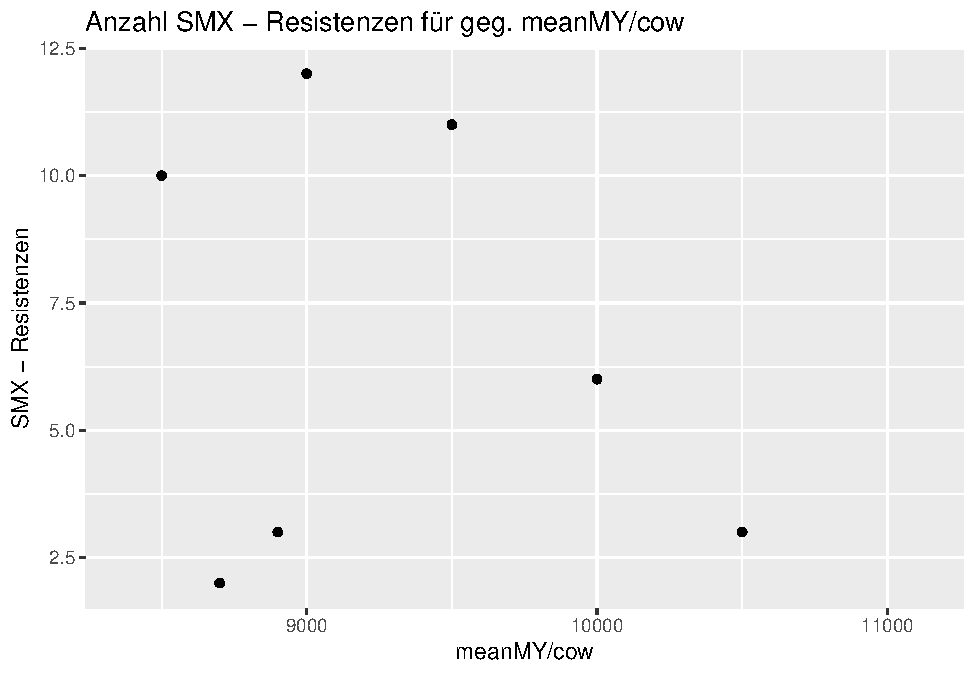
\includegraphics{NResistenzen_files/figure-latex/unnamed-chunk-6-10.pdf}

\begin{verbatim}
## [1] ""
## [1] "--------------------------------------------------------"
\end{verbatim}

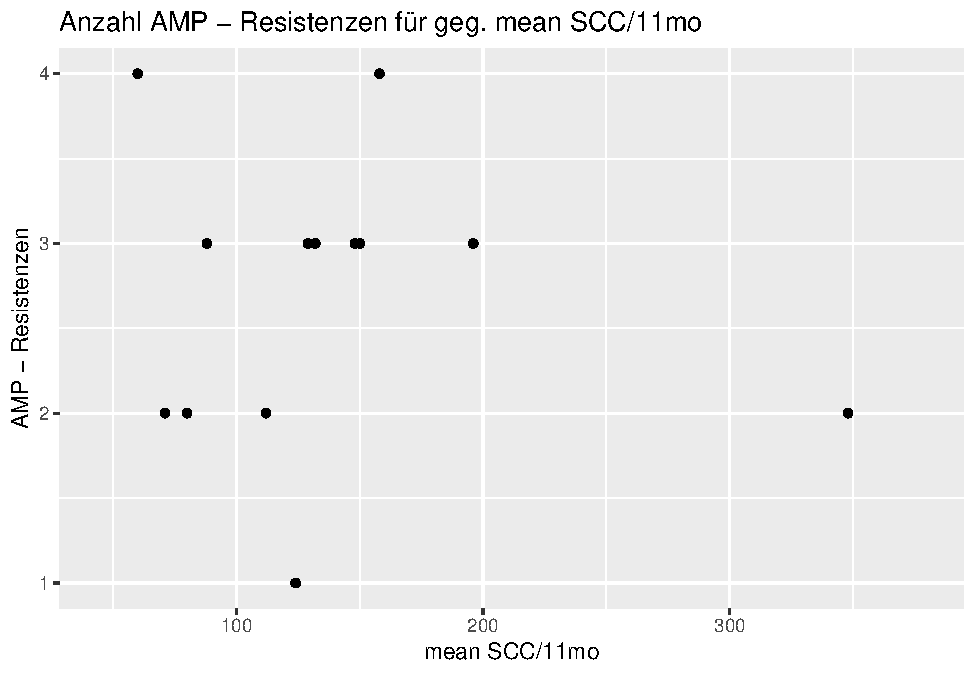
\includegraphics{NResistenzen_files/figure-latex/unnamed-chunk-6-11.pdf}

\begin{verbatim}
## [1] ""
\end{verbatim}

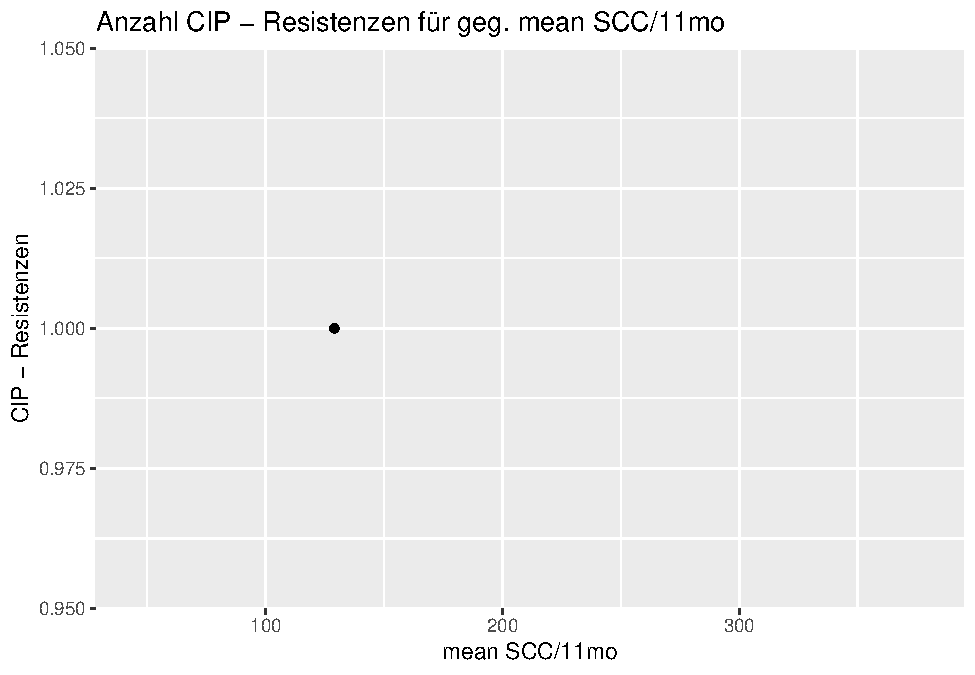
\includegraphics{NResistenzen_files/figure-latex/unnamed-chunk-6-12.pdf}

\begin{verbatim}
## [1] ""
\end{verbatim}

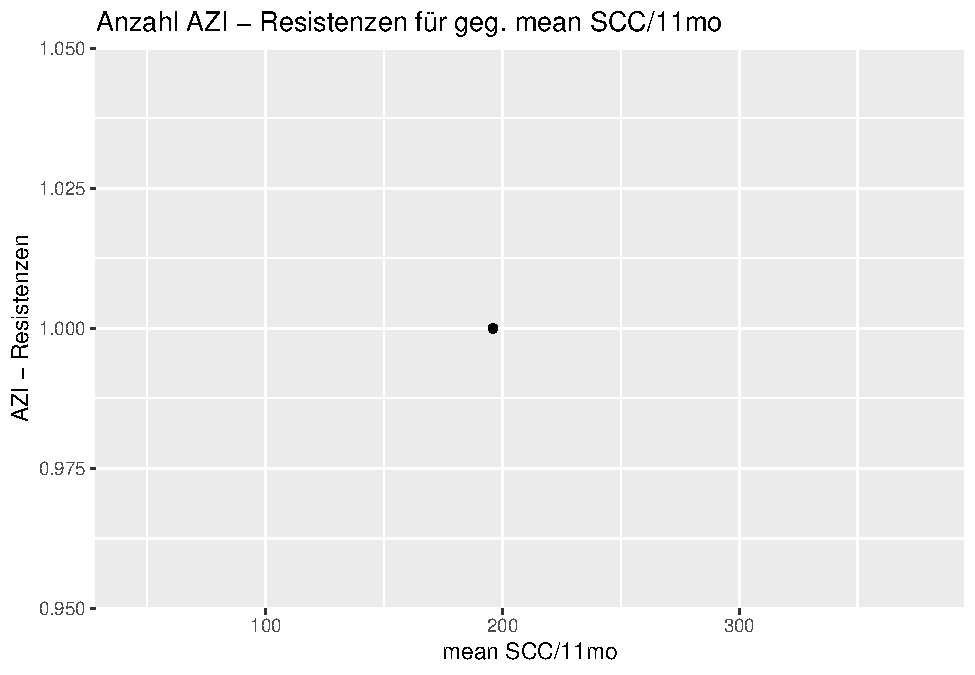
\includegraphics{NResistenzen_files/figure-latex/unnamed-chunk-6-13.pdf}

\begin{verbatim}
## [1] ""
\end{verbatim}

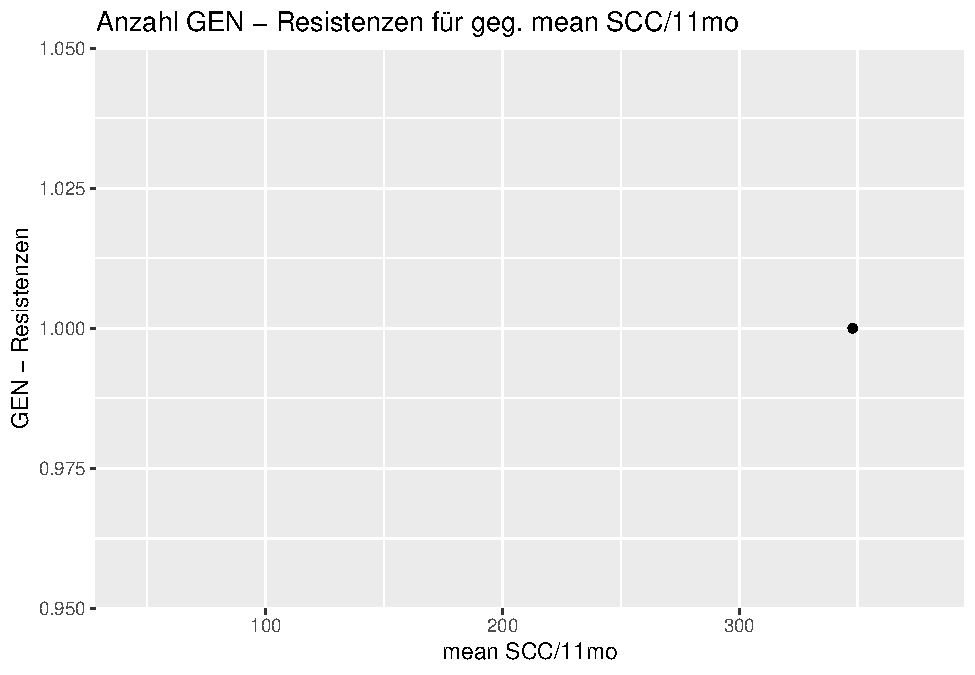
\includegraphics{NResistenzen_files/figure-latex/unnamed-chunk-6-14.pdf}

\begin{verbatim}
## [1] ""
\end{verbatim}

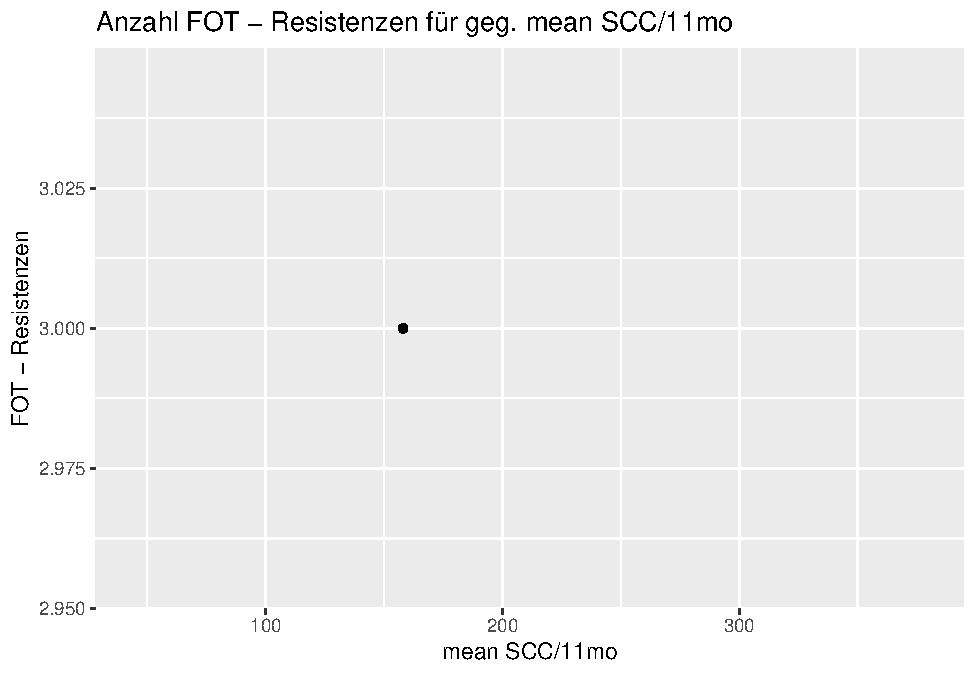
\includegraphics{NResistenzen_files/figure-latex/unnamed-chunk-6-15.pdf}

\begin{verbatim}
## [1] ""
\end{verbatim}

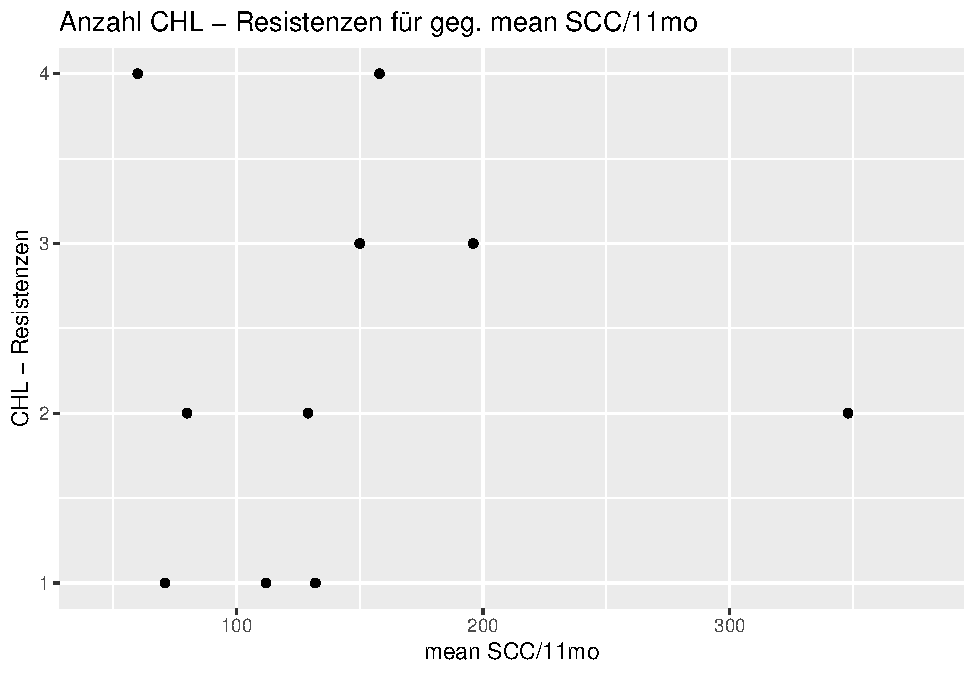
\includegraphics{NResistenzen_files/figure-latex/unnamed-chunk-6-16.pdf}

\begin{verbatim}
## [1] ""
\end{verbatim}

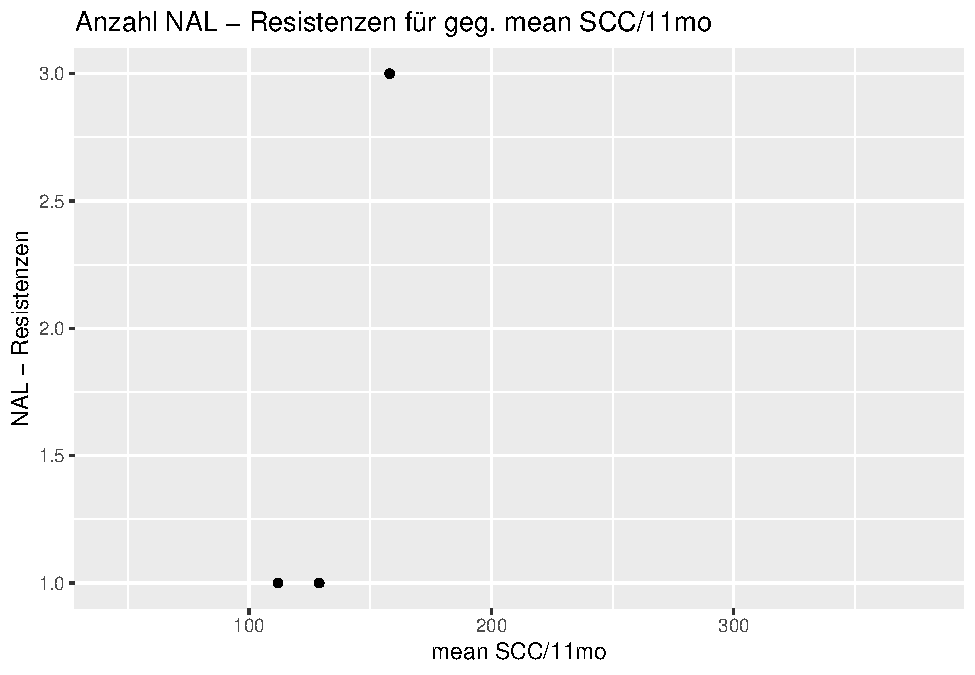
\includegraphics{NResistenzen_files/figure-latex/unnamed-chunk-6-17.pdf}

\begin{verbatim}
## [1] ""
\end{verbatim}

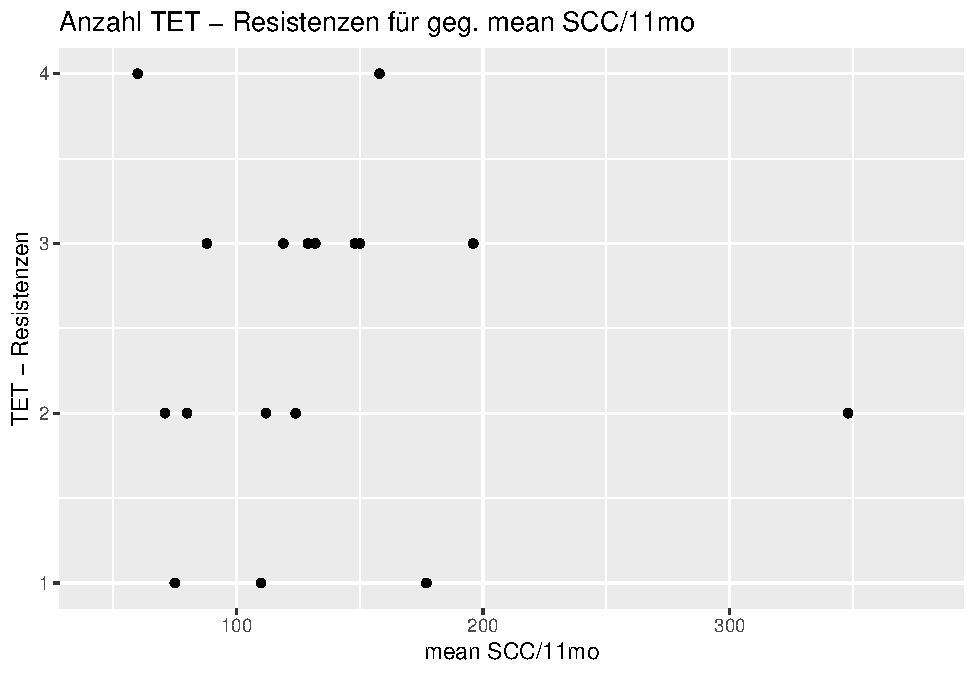
\includegraphics{NResistenzen_files/figure-latex/unnamed-chunk-6-18.pdf}

\begin{verbatim}
## [1] ""
\end{verbatim}

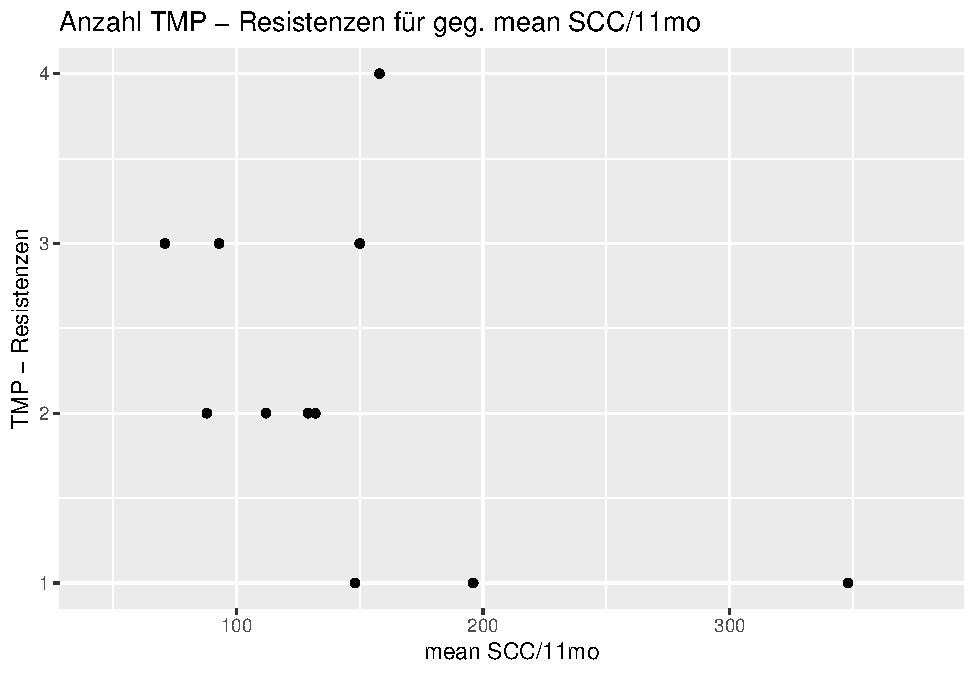
\includegraphics{NResistenzen_files/figure-latex/unnamed-chunk-6-19.pdf}

\begin{verbatim}
## [1] ""
\end{verbatim}

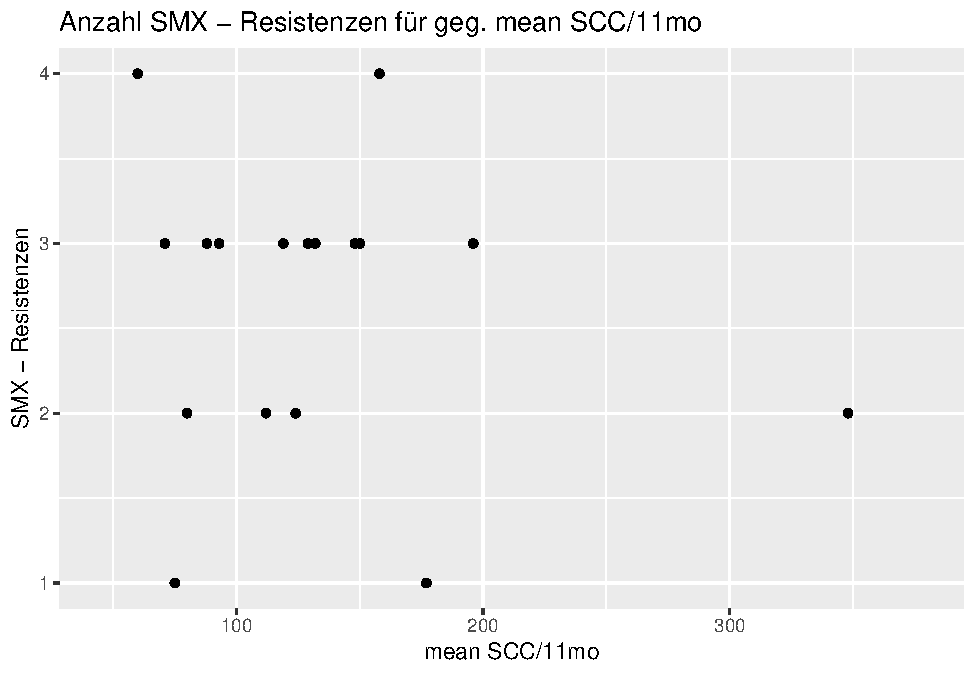
\includegraphics{NResistenzen_files/figure-latex/unnamed-chunk-6-20.pdf}

\begin{verbatim}
## [1] ""
## [1] "--------------------------------------------------------"
\end{verbatim}

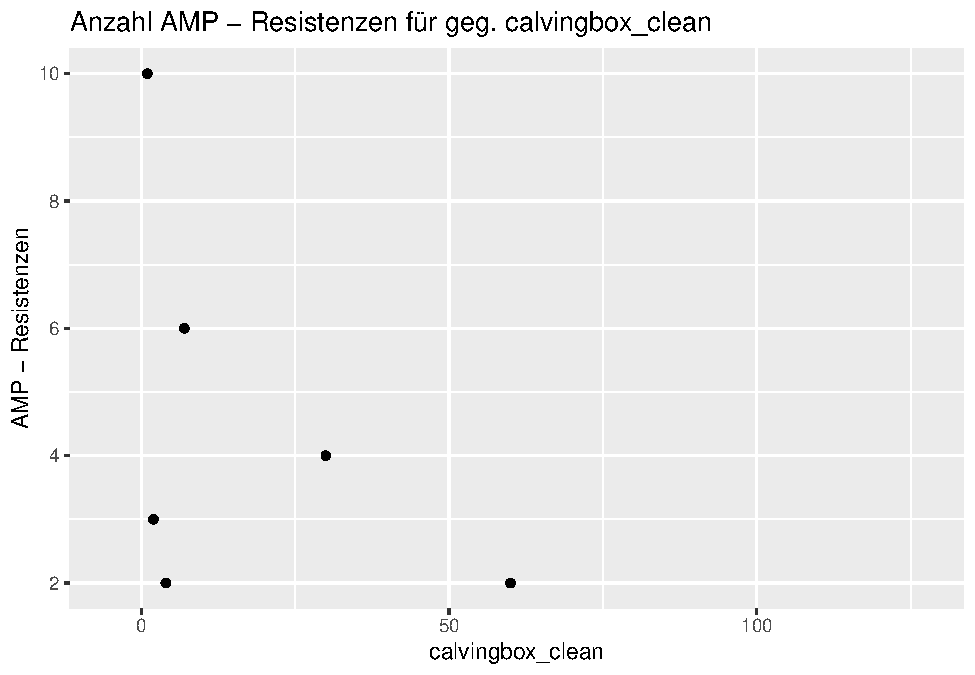
\includegraphics{NResistenzen_files/figure-latex/unnamed-chunk-6-21.pdf}

\begin{verbatim}
## [1] ""
\end{verbatim}

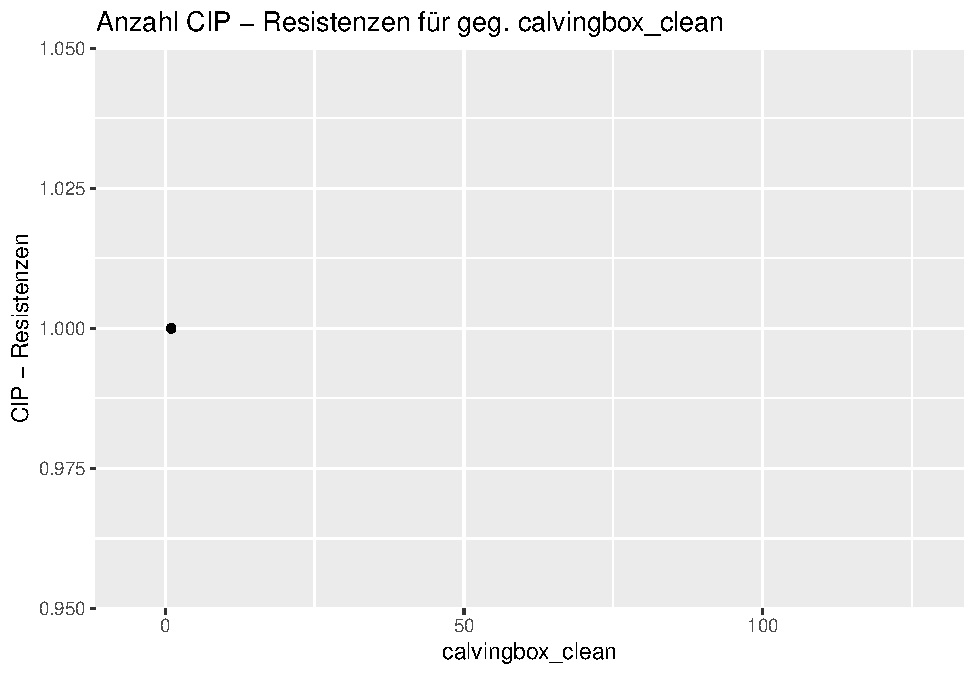
\includegraphics{NResistenzen_files/figure-latex/unnamed-chunk-6-22.pdf}

\begin{verbatim}
## [1] ""
\end{verbatim}

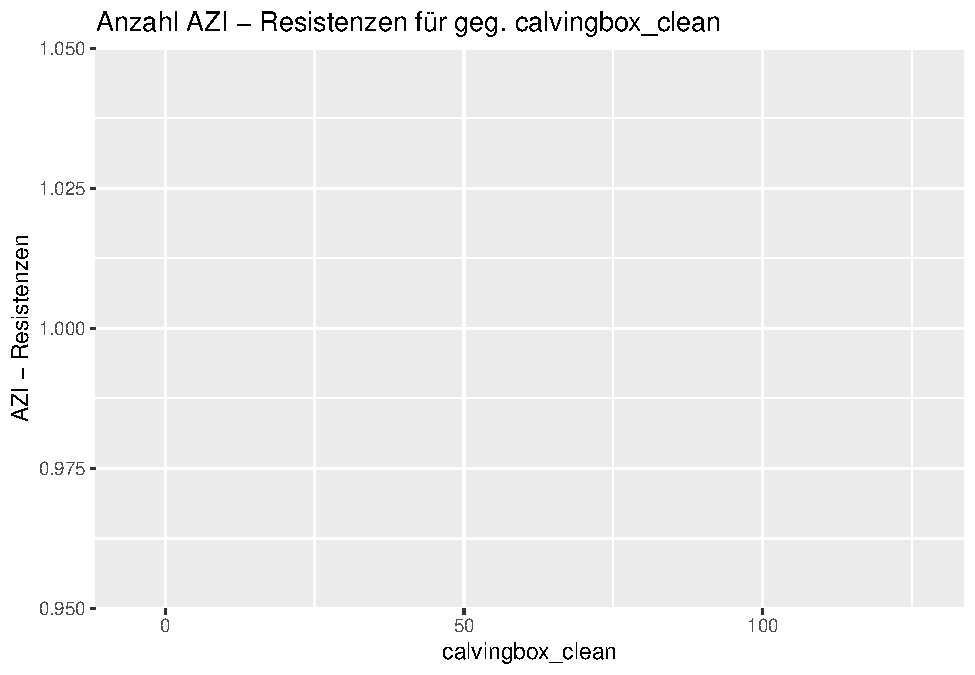
\includegraphics{NResistenzen_files/figure-latex/unnamed-chunk-6-23.pdf}

\begin{verbatim}
## [1] ""
\end{verbatim}

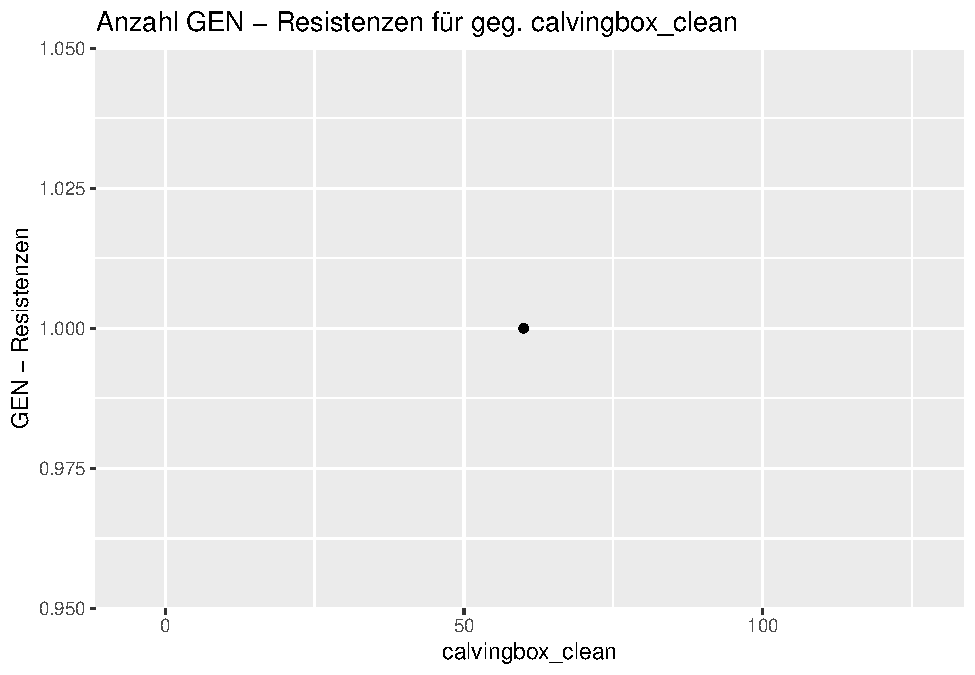
\includegraphics{NResistenzen_files/figure-latex/unnamed-chunk-6-24.pdf}

\begin{verbatim}
## [1] ""
\end{verbatim}

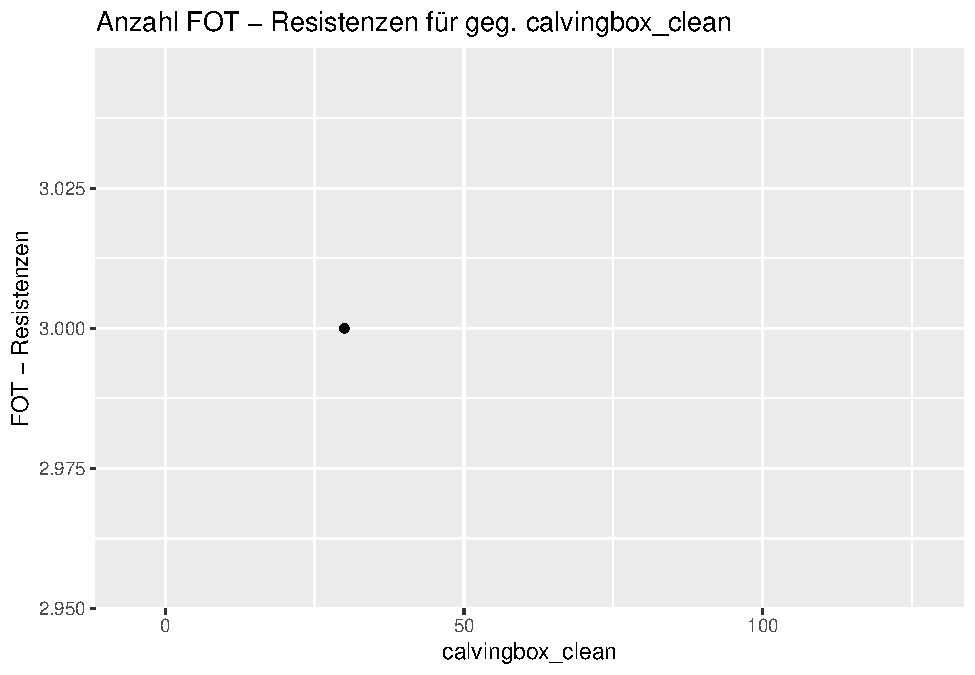
\includegraphics{NResistenzen_files/figure-latex/unnamed-chunk-6-25.pdf}

\begin{verbatim}
## [1] ""
\end{verbatim}

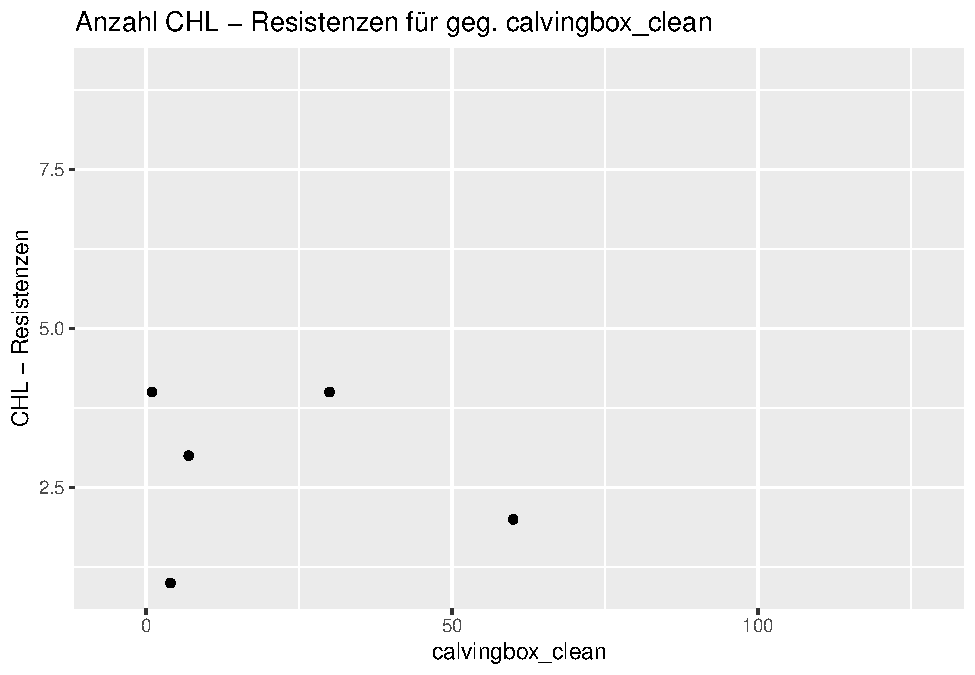
\includegraphics{NResistenzen_files/figure-latex/unnamed-chunk-6-26.pdf}

\begin{verbatim}
## [1] ""
\end{verbatim}

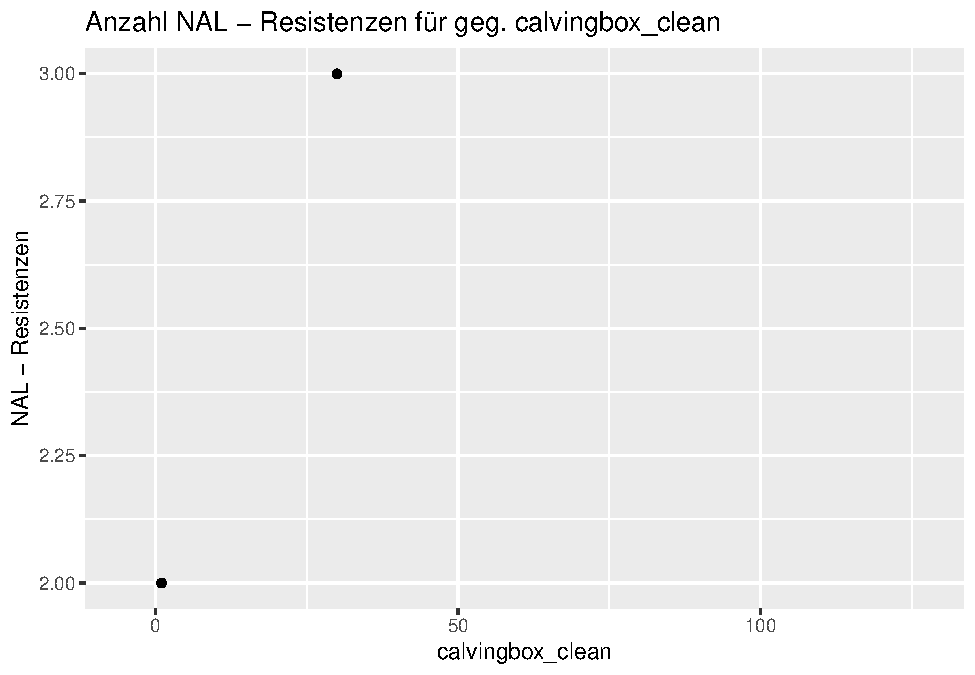
\includegraphics{NResistenzen_files/figure-latex/unnamed-chunk-6-27.pdf}

\begin{verbatim}
## [1] ""
\end{verbatim}

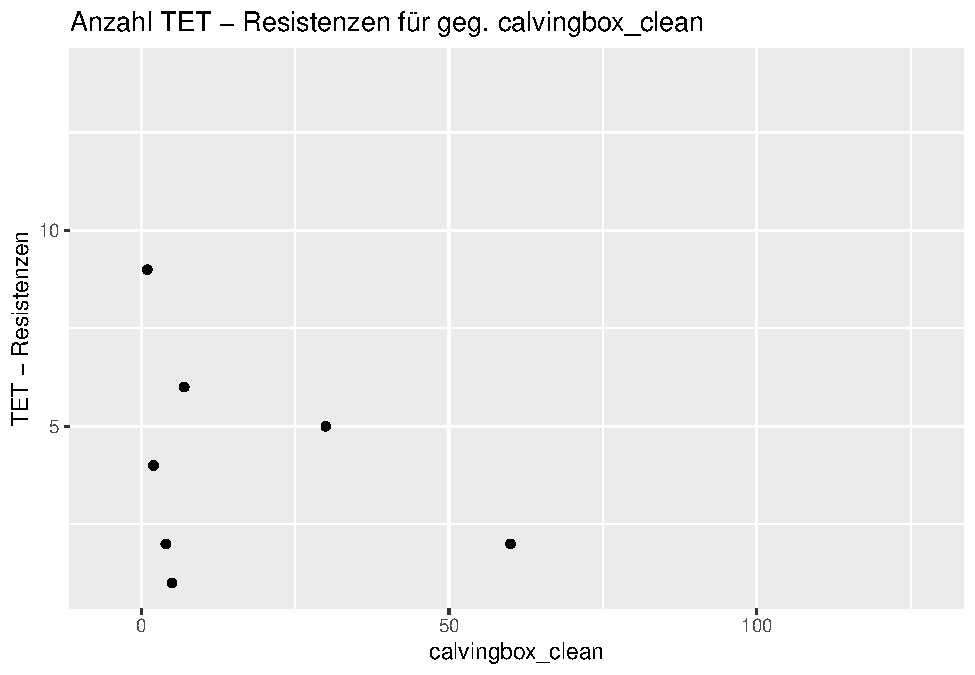
\includegraphics{NResistenzen_files/figure-latex/unnamed-chunk-6-28.pdf}

\begin{verbatim}
## [1] ""
\end{verbatim}

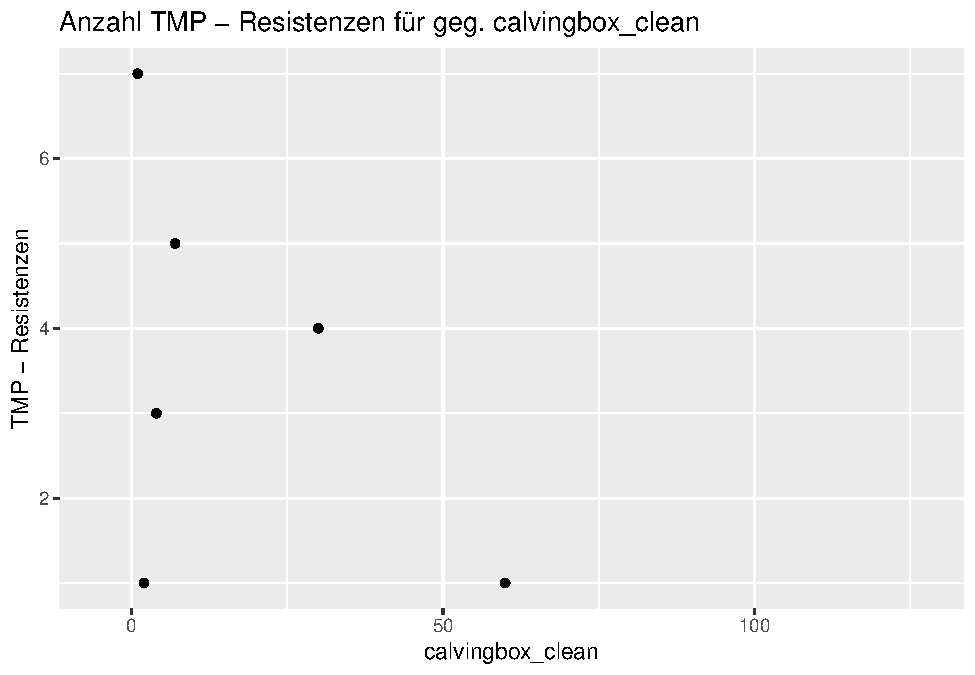
\includegraphics{NResistenzen_files/figure-latex/unnamed-chunk-6-29.pdf}

\begin{verbatim}
## [1] ""
\end{verbatim}

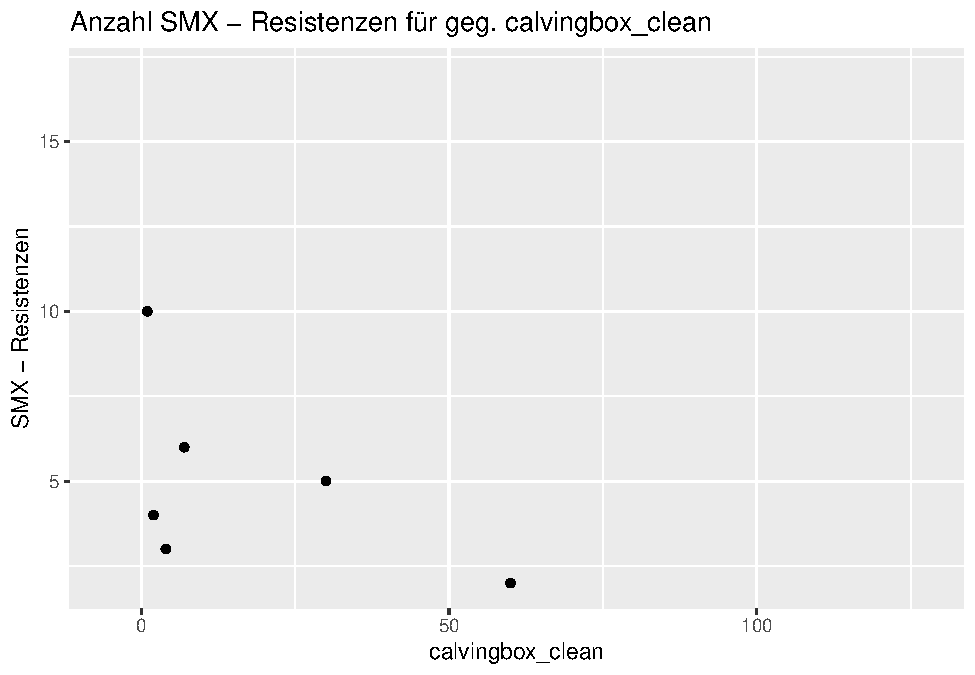
\includegraphics{NResistenzen_files/figure-latex/unnamed-chunk-6-30.pdf}

\begin{verbatim}
## [1] ""
## [1] "--------------------------------------------------------"
\end{verbatim}

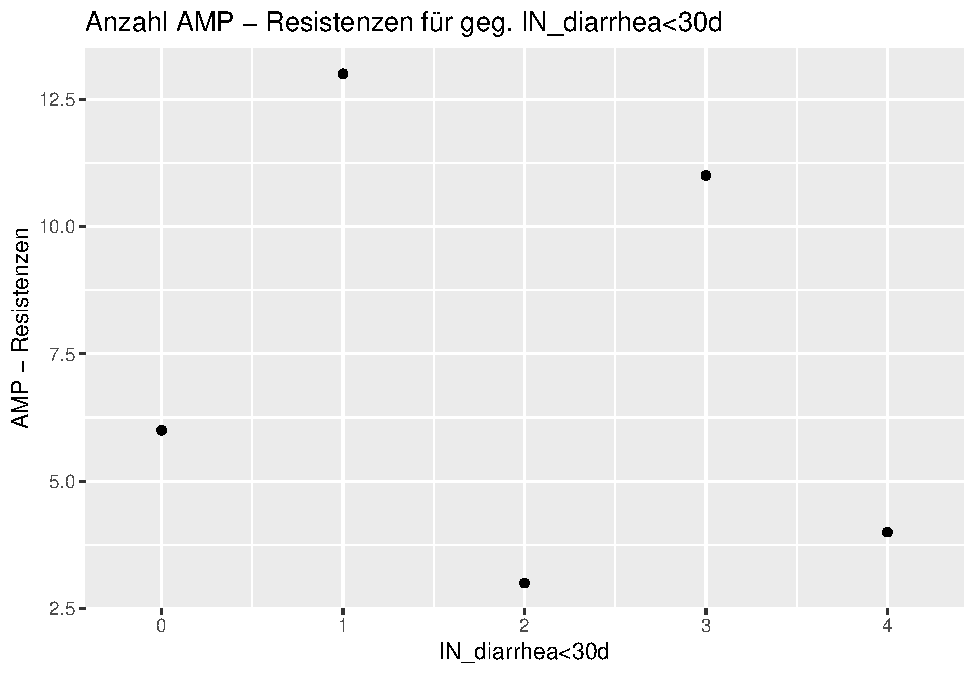
\includegraphics{NResistenzen_files/figure-latex/unnamed-chunk-6-31.pdf}

\begin{verbatim}
## [1] ""
\end{verbatim}

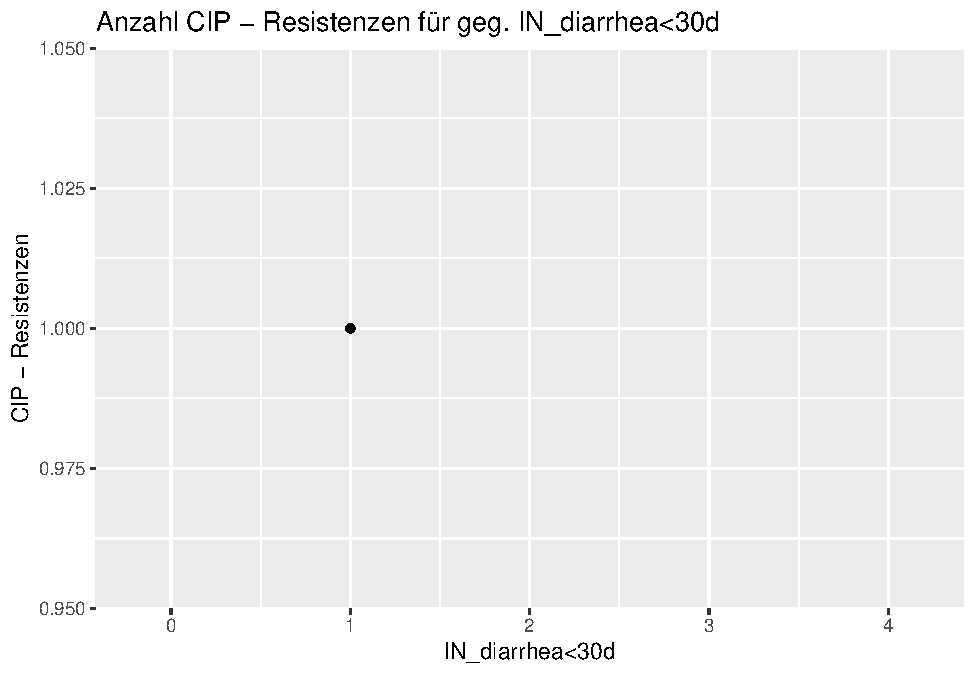
\includegraphics{NResistenzen_files/figure-latex/unnamed-chunk-6-32.pdf}

\begin{verbatim}
## [1] ""
\end{verbatim}

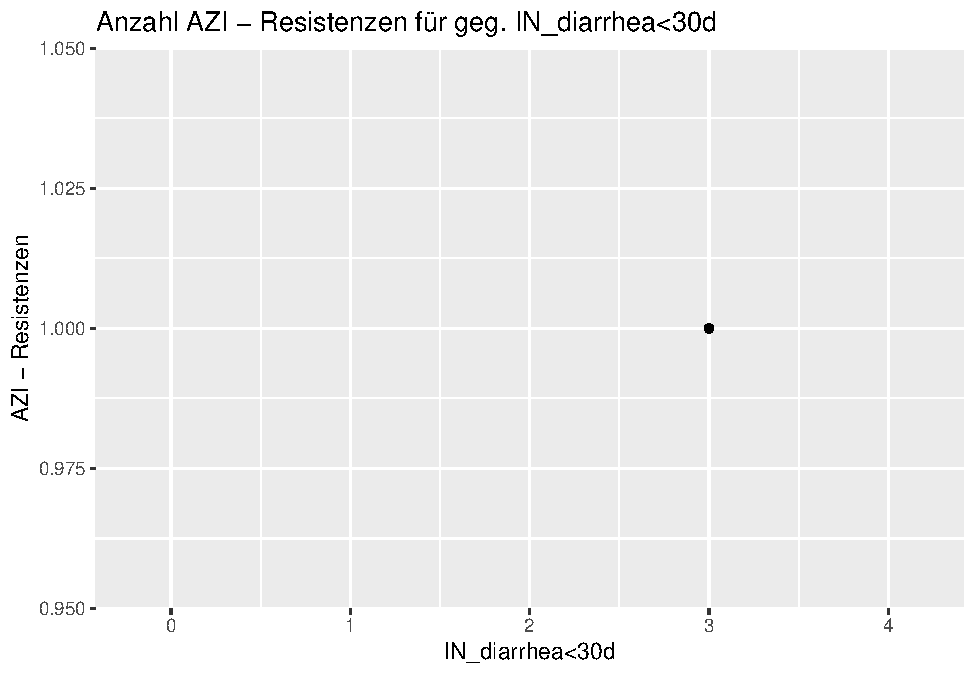
\includegraphics{NResistenzen_files/figure-latex/unnamed-chunk-6-33.pdf}

\begin{verbatim}
## [1] ""
\end{verbatim}

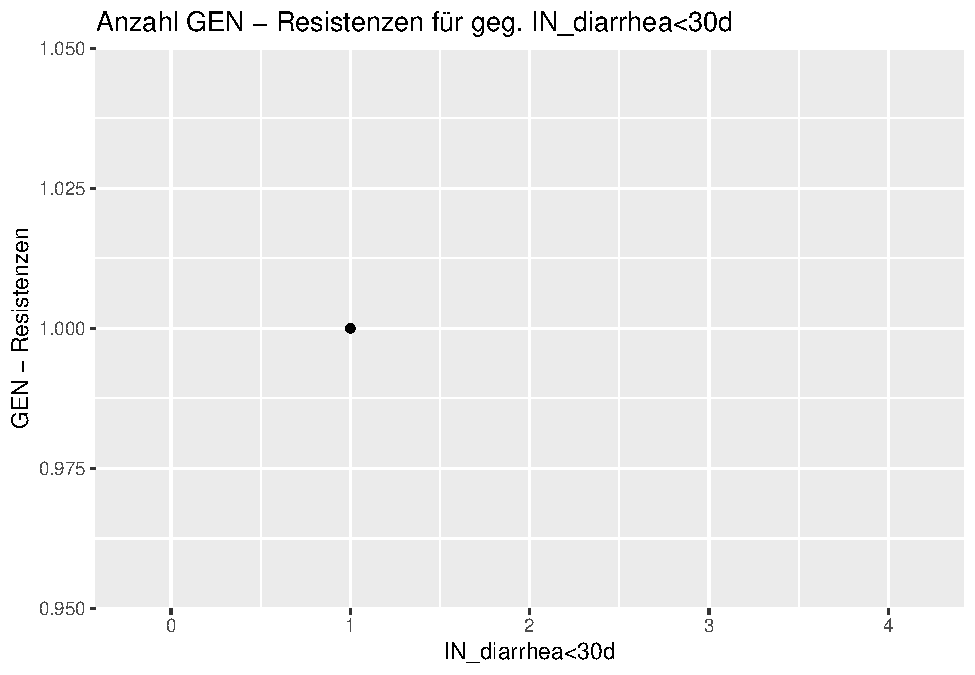
\includegraphics{NResistenzen_files/figure-latex/unnamed-chunk-6-34.pdf}

\begin{verbatim}
## [1] ""
\end{verbatim}

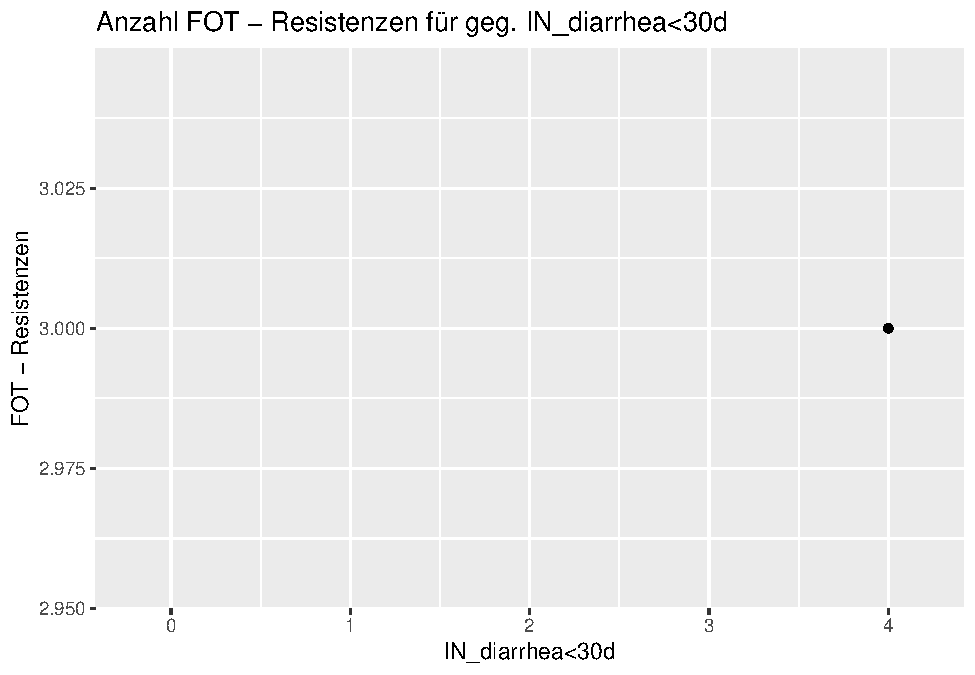
\includegraphics{NResistenzen_files/figure-latex/unnamed-chunk-6-35.pdf}

\begin{verbatim}
## [1] ""
\end{verbatim}

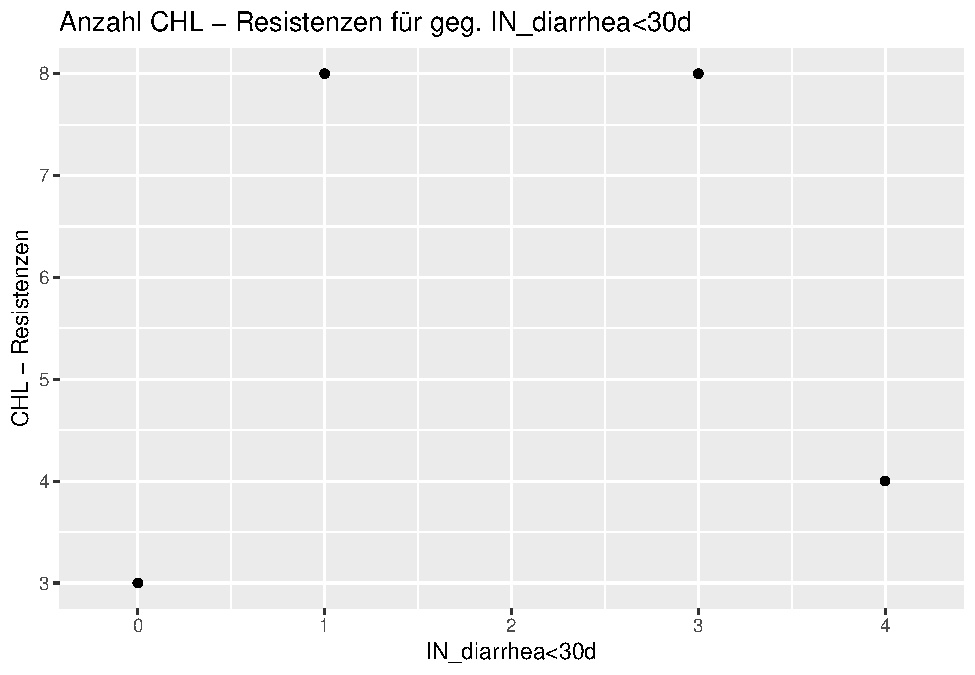
\includegraphics{NResistenzen_files/figure-latex/unnamed-chunk-6-36.pdf}

\begin{verbatim}
## [1] ""
\end{verbatim}

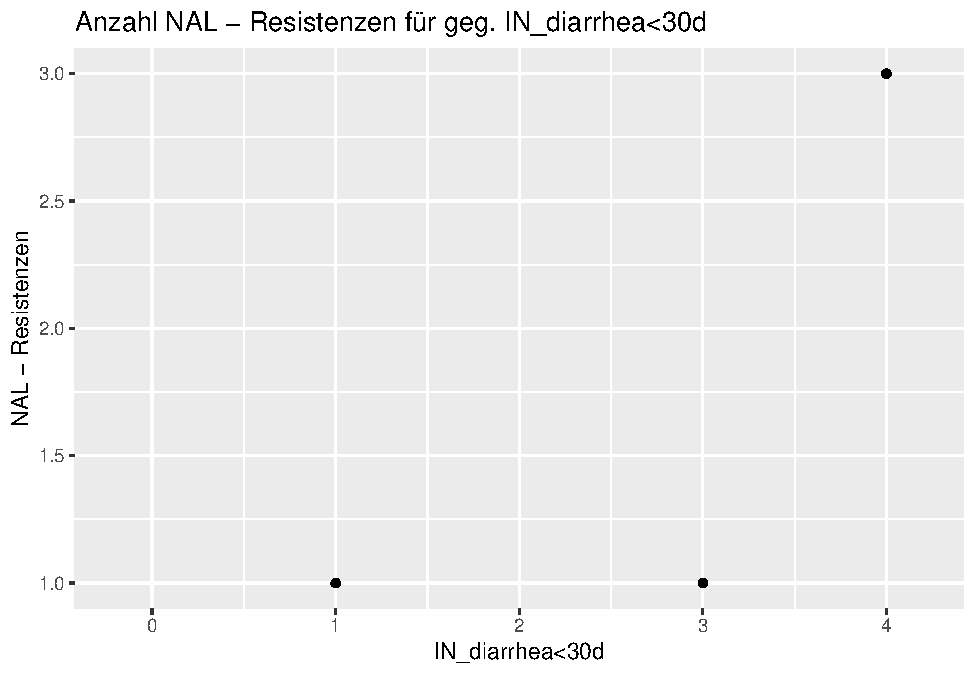
\includegraphics{NResistenzen_files/figure-latex/unnamed-chunk-6-37.pdf}

\begin{verbatim}
## [1] ""
\end{verbatim}

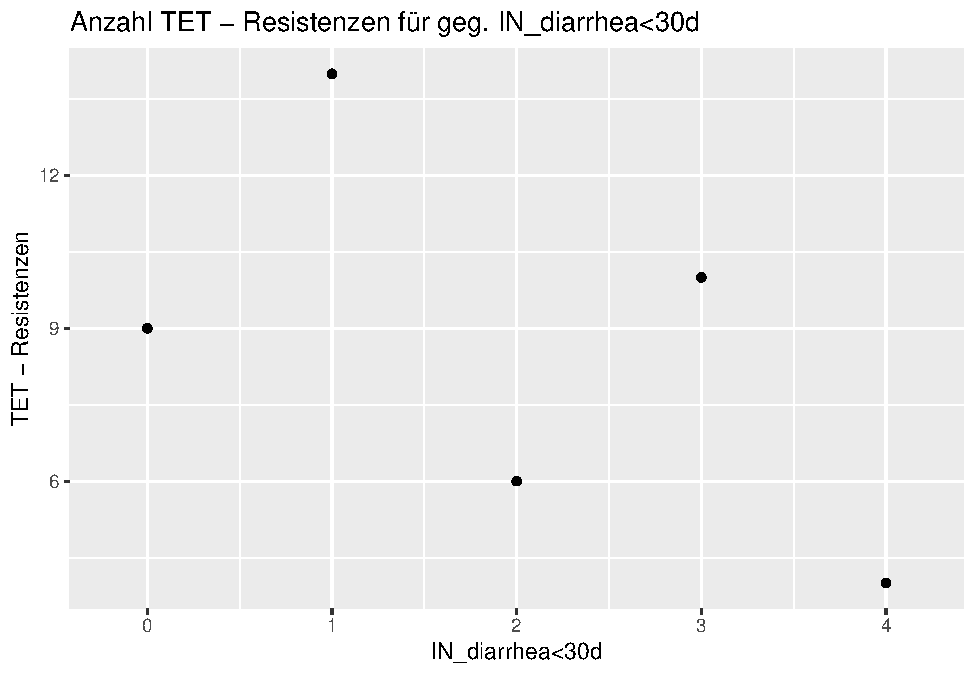
\includegraphics{NResistenzen_files/figure-latex/unnamed-chunk-6-38.pdf}

\begin{verbatim}
## [1] ""
\end{verbatim}

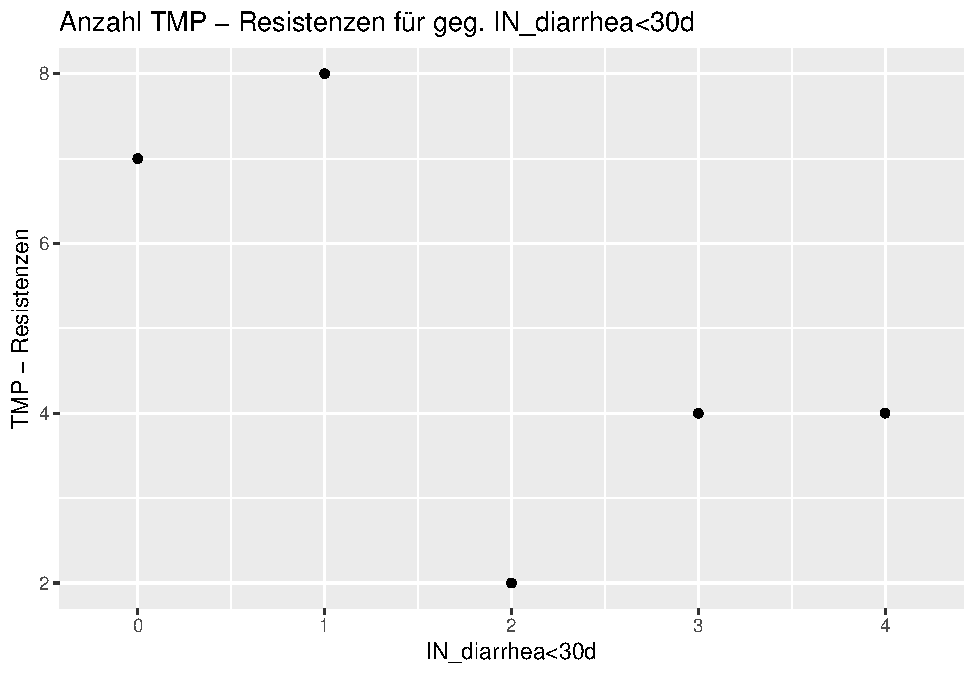
\includegraphics{NResistenzen_files/figure-latex/unnamed-chunk-6-39.pdf}

\begin{verbatim}
## [1] ""
\end{verbatim}

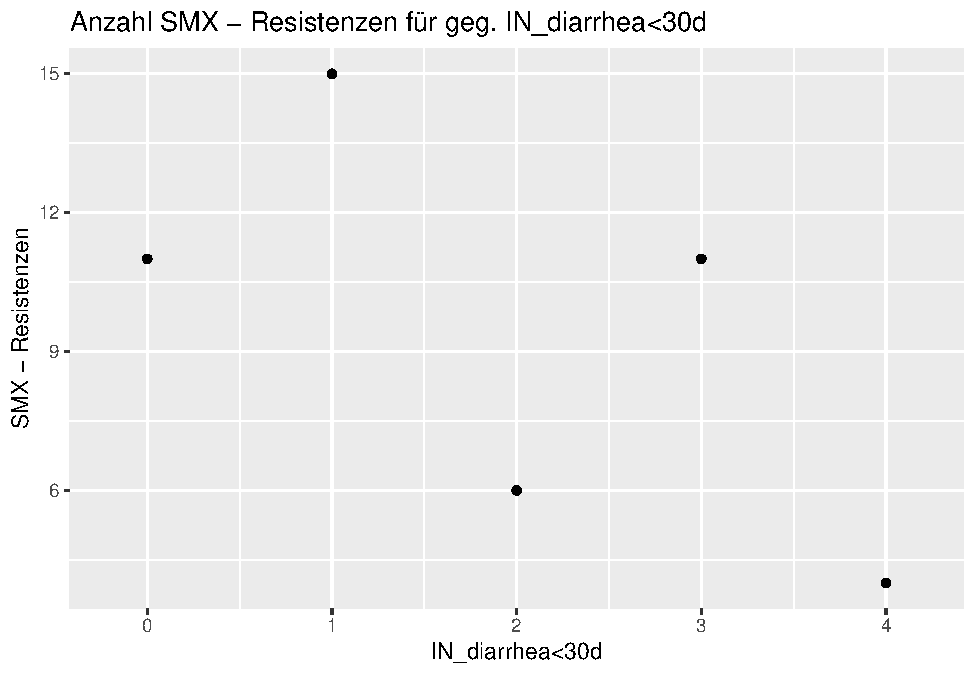
\includegraphics{NResistenzen_files/figure-latex/unnamed-chunk-6-40.pdf}

\begin{verbatim}
## [1] ""
## [1] "--------------------------------------------------------"
\end{verbatim}

Ungeschichtet: Resistenzen scheinen tendenziell zu

\begin{itemize}
\tightlist
\item
  steigen mit MY.group
\item
  fallen mit SCC.group, CBC.group
\item
  ? mit DIA.group
\end{itemize}

Eine Regression sagt mehr.

\hypertarget{binuxe4re-und-nominale-unabhuxe4ngige-variablen}{%
\section{Binäre und Nominale Unabhängige
Variablen}\label{binuxe4re-und-nominale-unabhuxe4ngige-variablen}}

\hypertarget{anzahl-resistenzen}{%
\subsection{Anzahl Resistenzen}\label{anzahl-resistenzen}}

\begin{Shaded}
\begin{Highlighting}[]
\CommentTok{# NA warnings interessieren nicht}

\CommentTok{# untersuchte binäre und nominale Variablen }

\CommentTok{### neue binäre oder nominale hier dazufügen : }\AlertTok{###}
\NormalTok{bin_nom <-}\StringTok{ }\KeywordTok{c}\NormalTok{(}\StringTok{"WM.group"}\NormalTok{, }\StringTok{"OLS.group"}\NormalTok{,}\StringTok{"IAC.group"}\NormalTok{,   }\StringTok{"HSC.group"}\NormalTok{)       }

\ControlFlowTok{for}\NormalTok{( group }\ControlFlowTok{in}\NormalTok{ bin_nom )\{}
  \ControlFlowTok{for}\NormalTok{( antib }\ControlFlowTok{in} \KeywordTok{c}\NormalTok{(}\StringTok{"AMP"}\NormalTok{,}\StringTok{"CIP"}\NormalTok{,}\StringTok{"AZI"}\NormalTok{,}\StringTok{"GEN"}\NormalTok{,}\StringTok{"FOT"}\NormalTok{,}\StringTok{"CHL"}\NormalTok{,}\StringTok{"NAL"}\NormalTok{,}\StringTok{"TET"}\NormalTok{,}\StringTok{"TMP"}\NormalTok{,}\StringTok{"SMX"}\NormalTok{) )\{}
    \CommentTok{#graphisch2(group,"für geg. Wert von",antib)  }
    \KeywordTok{graphisch2}\NormalTok{(group,}\StringTok{"für geg."}\NormalTok{,antib)  }
    \KeywordTok{print}\NormalTok{(}\StringTok{""}\NormalTok{)}
\NormalTok{  \} }
  \KeywordTok{print}\NormalTok{(}\StringTok{"--------------------------------------------------------"}\NormalTok{)}
\NormalTok{\}}
\end{Highlighting}
\end{Shaded}

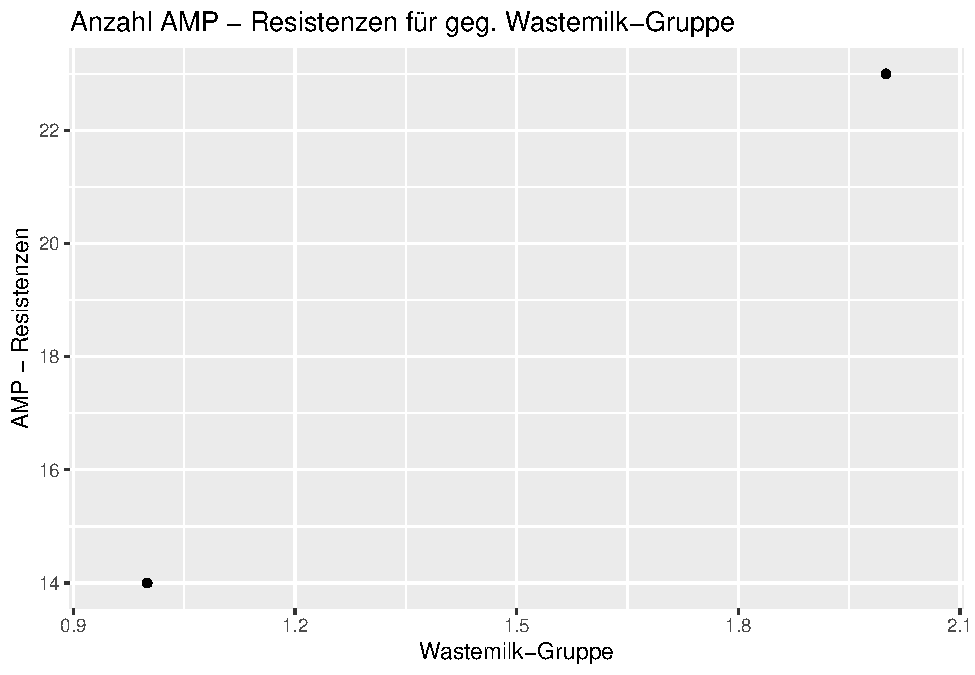
\includegraphics{NResistenzen_files/figure-latex/unnamed-chunk-7-1.pdf}

\begin{verbatim}
## [1] ""
\end{verbatim}

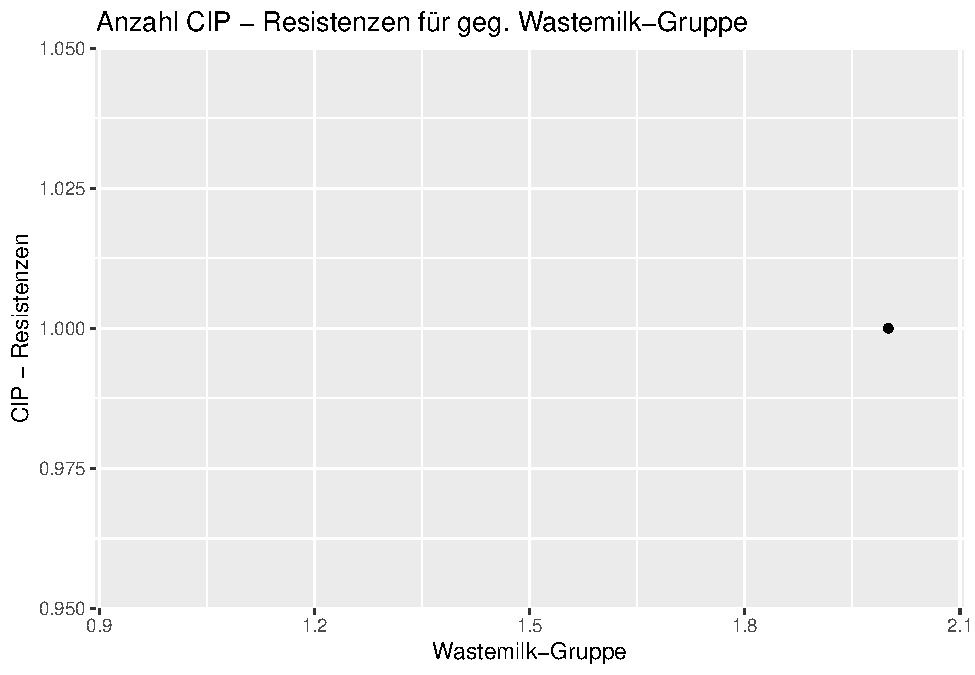
\includegraphics{NResistenzen_files/figure-latex/unnamed-chunk-7-2.pdf}

\begin{verbatim}
## [1] ""
\end{verbatim}

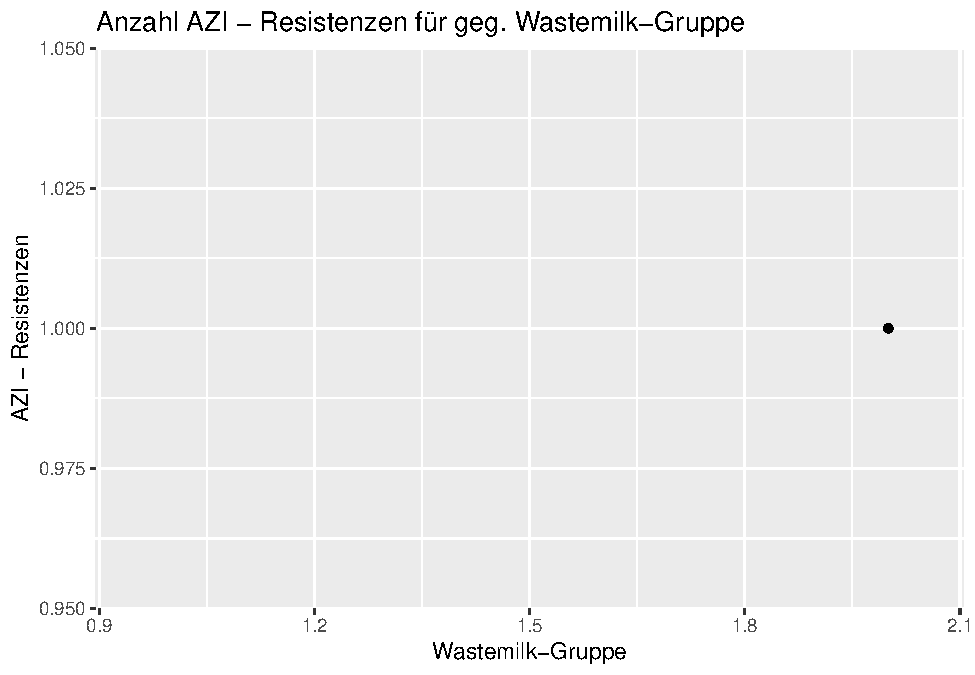
\includegraphics{NResistenzen_files/figure-latex/unnamed-chunk-7-3.pdf}

\begin{verbatim}
## [1] ""
\end{verbatim}

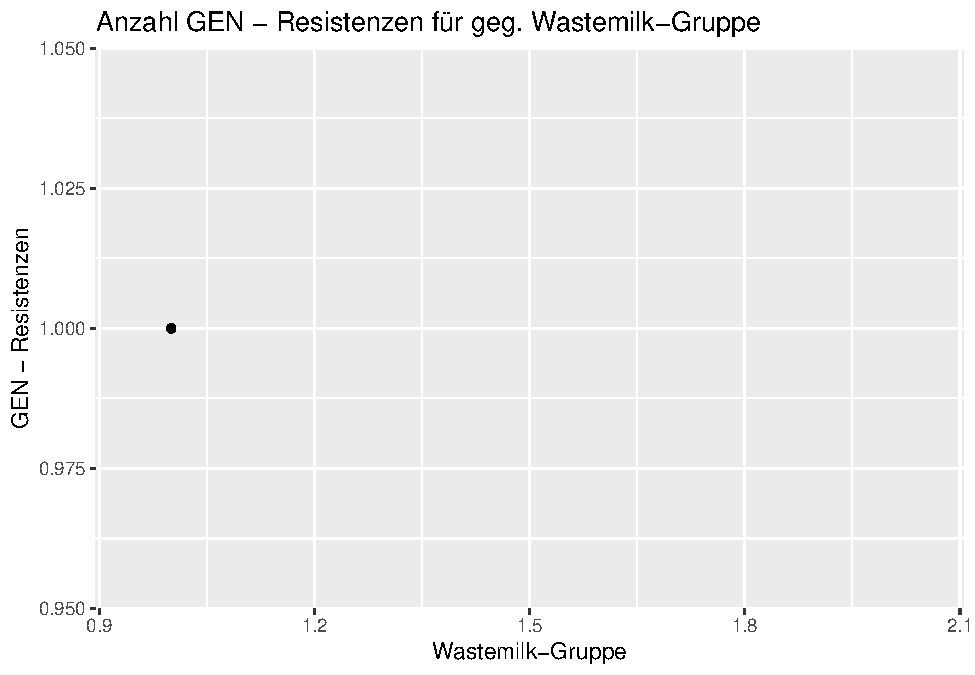
\includegraphics{NResistenzen_files/figure-latex/unnamed-chunk-7-4.pdf}

\begin{verbatim}
## [1] ""
\end{verbatim}

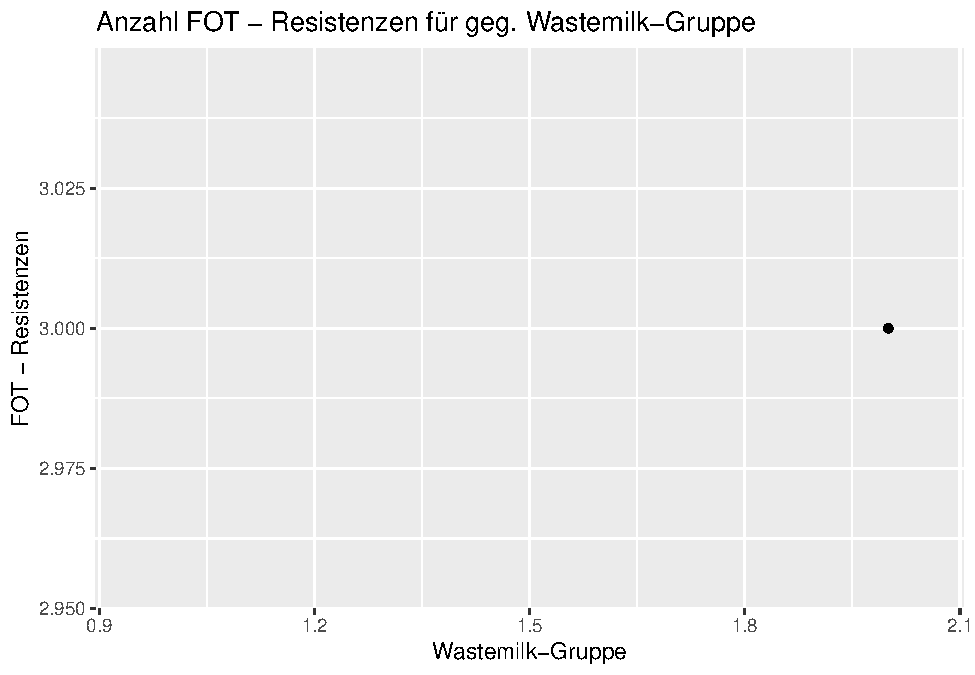
\includegraphics{NResistenzen_files/figure-latex/unnamed-chunk-7-5.pdf}

\begin{verbatim}
## [1] ""
\end{verbatim}

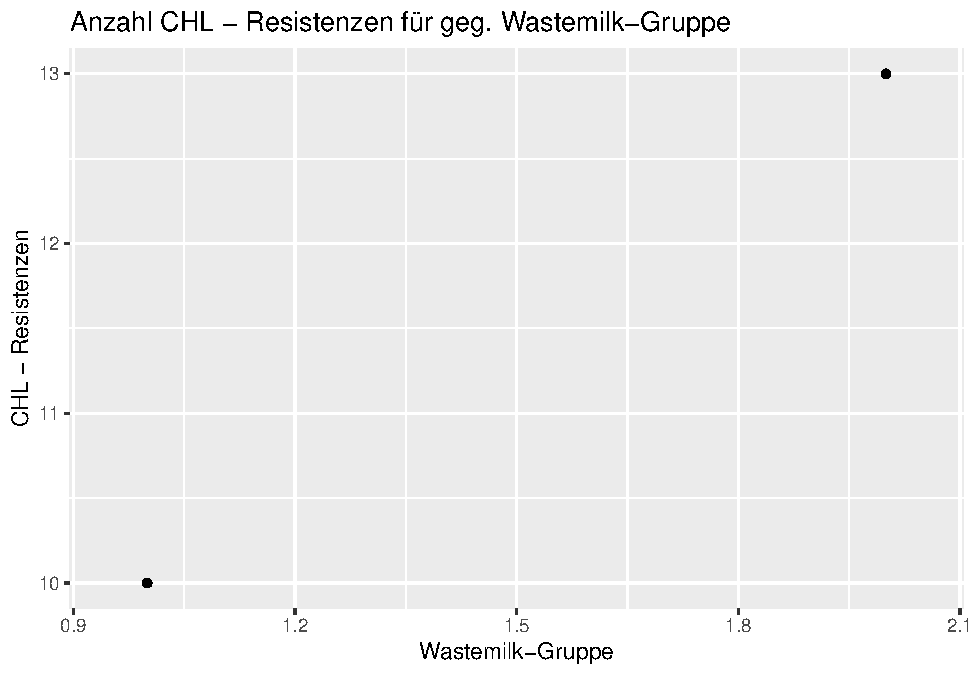
\includegraphics{NResistenzen_files/figure-latex/unnamed-chunk-7-6.pdf}

\begin{verbatim}
## [1] ""
\end{verbatim}

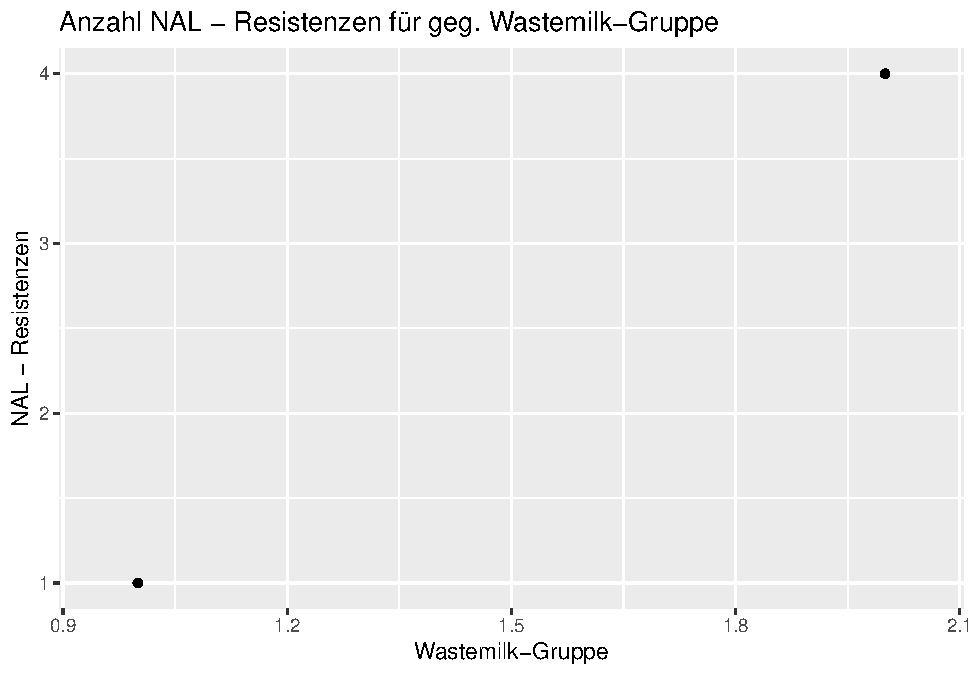
\includegraphics{NResistenzen_files/figure-latex/unnamed-chunk-7-7.pdf}

\begin{verbatim}
## [1] ""
\end{verbatim}

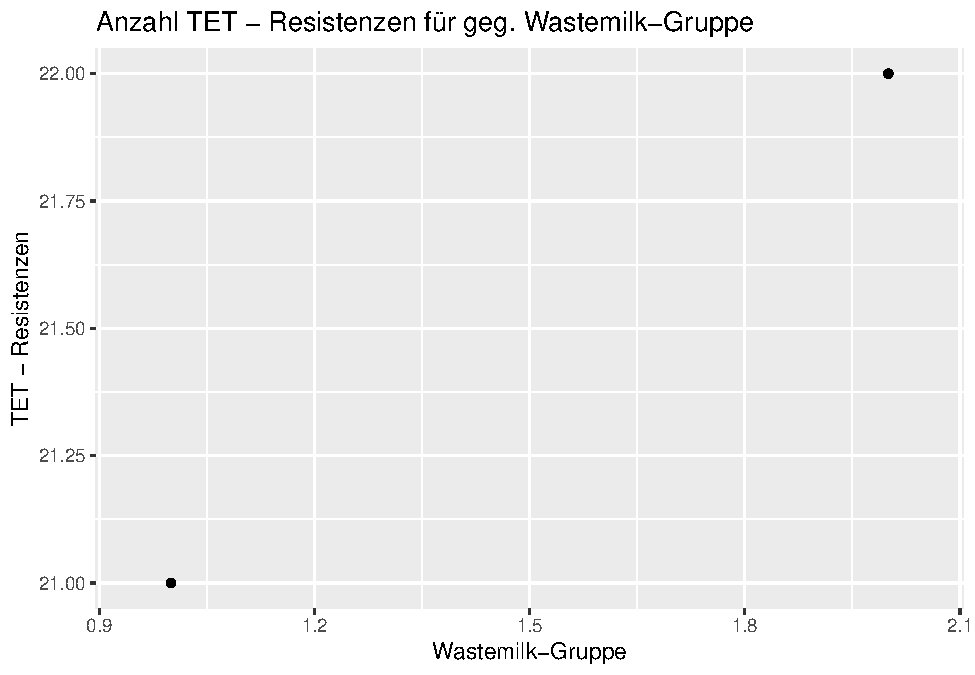
\includegraphics{NResistenzen_files/figure-latex/unnamed-chunk-7-8.pdf}

\begin{verbatim}
## [1] ""
\end{verbatim}

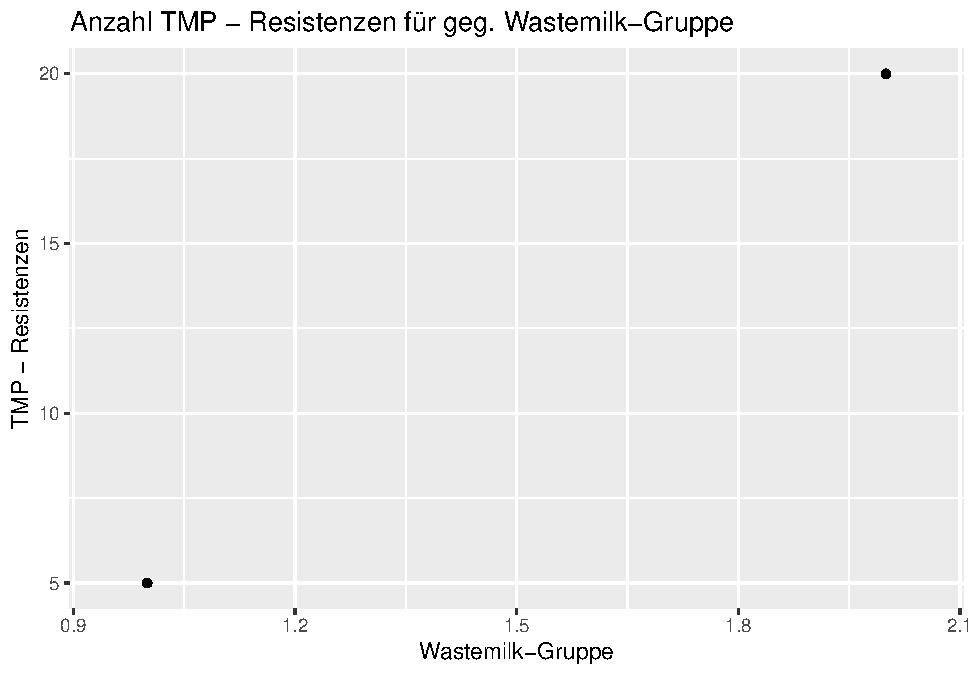
\includegraphics{NResistenzen_files/figure-latex/unnamed-chunk-7-9.pdf}

\begin{verbatim}
## [1] ""
\end{verbatim}

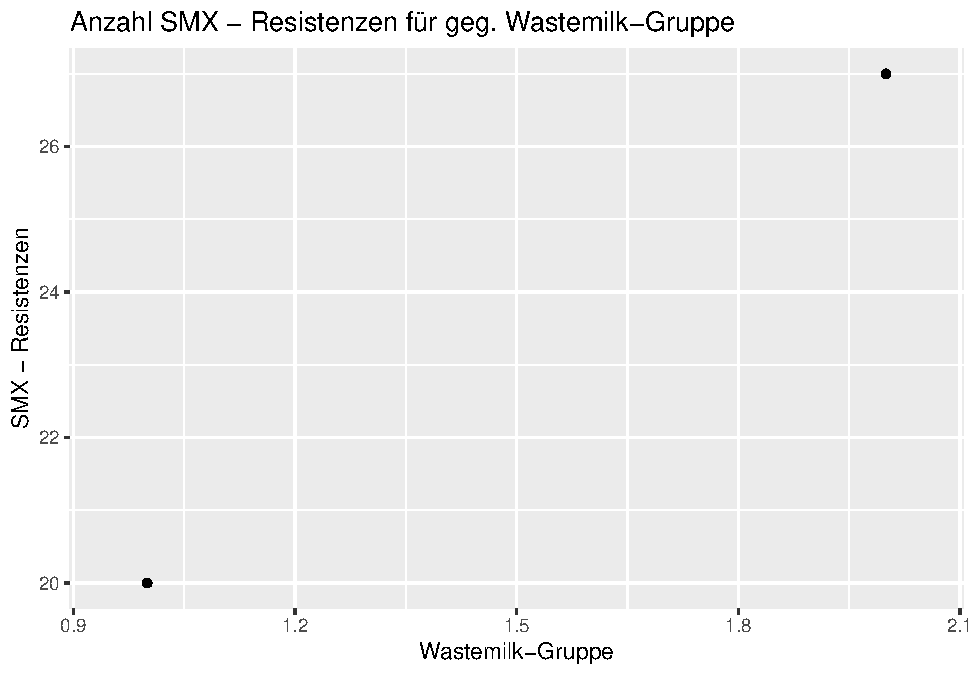
\includegraphics{NResistenzen_files/figure-latex/unnamed-chunk-7-10.pdf}

\begin{verbatim}
## [1] ""
## [1] "--------------------------------------------------------"
\end{verbatim}

\includegraphics{NResistenzen_files/figure-latex/unnamed-chunk-7-11.pdf}

\begin{verbatim}
## [1] ""
\end{verbatim}

\includegraphics{NResistenzen_files/figure-latex/unnamed-chunk-7-12.pdf}

\begin{verbatim}
## [1] ""
\end{verbatim}

\includegraphics{NResistenzen_files/figure-latex/unnamed-chunk-7-13.pdf}

\begin{verbatim}
## [1] ""
\end{verbatim}

\includegraphics{NResistenzen_files/figure-latex/unnamed-chunk-7-14.pdf}

\begin{verbatim}
## [1] ""
\end{verbatim}

\includegraphics{NResistenzen_files/figure-latex/unnamed-chunk-7-15.pdf}

\begin{verbatim}
## [1] ""
\end{verbatim}

\includegraphics{NResistenzen_files/figure-latex/unnamed-chunk-7-16.pdf}

\begin{verbatim}
## [1] ""
\end{verbatim}

\includegraphics{NResistenzen_files/figure-latex/unnamed-chunk-7-17.pdf}

\begin{verbatim}
## [1] ""
\end{verbatim}

\includegraphics{NResistenzen_files/figure-latex/unnamed-chunk-7-18.pdf}

\begin{verbatim}
## [1] ""
\end{verbatim}

\includegraphics{NResistenzen_files/figure-latex/unnamed-chunk-7-19.pdf}

\begin{verbatim}
## [1] ""
\end{verbatim}

\includegraphics{NResistenzen_files/figure-latex/unnamed-chunk-7-20.pdf}

\begin{verbatim}
## [1] ""
## [1] "--------------------------------------------------------"
\end{verbatim}

\includegraphics{NResistenzen_files/figure-latex/unnamed-chunk-7-21.pdf}

\begin{verbatim}
## [1] ""
\end{verbatim}

\includegraphics{NResistenzen_files/figure-latex/unnamed-chunk-7-22.pdf}

\begin{verbatim}
## [1] ""
\end{verbatim}

\includegraphics{NResistenzen_files/figure-latex/unnamed-chunk-7-23.pdf}

\begin{verbatim}
## [1] ""
\end{verbatim}

\includegraphics{NResistenzen_files/figure-latex/unnamed-chunk-7-24.pdf}

\begin{verbatim}
## [1] ""
\end{verbatim}

\includegraphics{NResistenzen_files/figure-latex/unnamed-chunk-7-25.pdf}

\begin{verbatim}
## [1] ""
\end{verbatim}

\includegraphics{NResistenzen_files/figure-latex/unnamed-chunk-7-26.pdf}

\begin{verbatim}
## [1] ""
\end{verbatim}

\includegraphics{NResistenzen_files/figure-latex/unnamed-chunk-7-27.pdf}

\begin{verbatim}
## [1] ""
\end{verbatim}

\includegraphics{NResistenzen_files/figure-latex/unnamed-chunk-7-28.pdf}

\begin{verbatim}
## [1] ""
\end{verbatim}

\includegraphics{NResistenzen_files/figure-latex/unnamed-chunk-7-29.pdf}

\begin{verbatim}
## [1] ""
\end{verbatim}

\includegraphics{NResistenzen_files/figure-latex/unnamed-chunk-7-30.pdf}

\begin{verbatim}
## [1] ""
## [1] "--------------------------------------------------------"
\end{verbatim}

\includegraphics{NResistenzen_files/figure-latex/unnamed-chunk-7-31.pdf}

\begin{verbatim}
## [1] ""
\end{verbatim}

\includegraphics{NResistenzen_files/figure-latex/unnamed-chunk-7-32.pdf}

\begin{verbatim}
## [1] ""
\end{verbatim}

\includegraphics{NResistenzen_files/figure-latex/unnamed-chunk-7-33.pdf}

\begin{verbatim}
## [1] ""
\end{verbatim}

\includegraphics{NResistenzen_files/figure-latex/unnamed-chunk-7-34.pdf}

\begin{verbatim}
## [1] ""
\end{verbatim}

\includegraphics{NResistenzen_files/figure-latex/unnamed-chunk-7-35.pdf}

\begin{verbatim}
## [1] ""
\end{verbatim}

\includegraphics{NResistenzen_files/figure-latex/unnamed-chunk-7-36.pdf}

\begin{verbatim}
## [1] ""
\end{verbatim}

\includegraphics{NResistenzen_files/figure-latex/unnamed-chunk-7-37.pdf}

\begin{verbatim}
## [1] ""
\end{verbatim}

\includegraphics{NResistenzen_files/figure-latex/unnamed-chunk-7-38.pdf}

\begin{verbatim}
## [1] ""
\end{verbatim}

\includegraphics{NResistenzen_files/figure-latex/unnamed-chunk-7-39.pdf}

\begin{verbatim}
## [1] ""
\end{verbatim}

\includegraphics{NResistenzen_files/figure-latex/unnamed-chunk-7-40.pdf}

\begin{verbatim}
## [1] ""
## [1] "--------------------------------------------------------"
\end{verbatim}

Ungeschichtet: Resistenzen scheinen zu

\begin{itemize}
\tightlist
\item
  steigen mit MY (das sahen wir schon aus den Verteilungen), OLS.group,
  tendenziell auch IAC.group
\item
  fallen bis HSC.group = 3, dann wieder etwas zu steigen (die Steigung
  von \(4\mapsto5\) scheint einleuchtend, da 5=0+2 und 4=1+2; man könnte
  \(4\leftrightarrow 5\) im plot vertauschen)
\item
  jedenfalls sind die Trends klarer als aus den Verteilungen. Eine
  Regression sagt nochmal mehr
\end{itemize}

\end{document}
